\documentclass[twoside]{book}

% Packages required by doxygen
\usepackage{fixltx2e}
\usepackage{calc}
\usepackage{doxygen}
\usepackage[export]{adjustbox} % also loads graphicx
\usepackage{graphicx}
\usepackage[utf8]{inputenc}
\usepackage{makeidx}
\usepackage{multicol}
\usepackage{multirow}
\PassOptionsToPackage{warn}{textcomp}
\usepackage{textcomp}
\usepackage[nointegrals]{wasysym}
\usepackage[table]{xcolor}

% Font selection
\usepackage[T1]{fontenc}
\usepackage[scaled=.90]{helvet}
\usepackage{courier}
\usepackage{amssymb}
\usepackage{sectsty}
\renewcommand{\familydefault}{\sfdefault}
\allsectionsfont{%
  \fontseries{bc}\selectfont%
  \color{darkgray}%
}
\renewcommand{\DoxyLabelFont}{%
  \fontseries{bc}\selectfont%
  \color{darkgray}%
}
\newcommand{\+}{\discretionary{\mbox{\scriptsize$\hookleftarrow$}}{}{}}

% Page & text layout
\usepackage{geometry}
\geometry{%
  a4paper,%
  top=2.5cm,%
  bottom=2.5cm,%
  left=2.5cm,%
  right=2.5cm%
}
\tolerance=750
\hfuzz=15pt
\hbadness=750
\setlength{\emergencystretch}{15pt}
\setlength{\parindent}{0cm}
\setlength{\parskip}{0.2cm}
\makeatletter
\renewcommand{\paragraph}{%
  \@startsection{paragraph}{4}{0ex}{-1.0ex}{1.0ex}{%
    \normalfont\normalsize\bfseries\SS@parafont%
  }%
}
\renewcommand{\subparagraph}{%
  \@startsection{subparagraph}{5}{0ex}{-1.0ex}{1.0ex}{%
    \normalfont\normalsize\bfseries\SS@subparafont%
  }%
}
\makeatother

% Headers & footers
\usepackage{fancyhdr}
\pagestyle{fancyplain}
\fancyhead[LE]{\fancyplain{}{\bfseries\thepage}}
\fancyhead[CE]{\fancyplain{}{}}
\fancyhead[RE]{\fancyplain{}{\bfseries\leftmark}}
\fancyhead[LO]{\fancyplain{}{\bfseries\rightmark}}
\fancyhead[CO]{\fancyplain{}{}}
\fancyhead[RO]{\fancyplain{}{\bfseries\thepage}}
\fancyfoot[LE]{\fancyplain{}{}}
\fancyfoot[CE]{\fancyplain{}{}}
\fancyfoot[RE]{\fancyplain{}{\bfseries\scriptsize Generated on Sun Nov 8 2015 21\+:06\+:02 for campeonatos polidesportivos by Doxygen }}
\fancyfoot[LO]{\fancyplain{}{\bfseries\scriptsize Generated on Sun Nov 8 2015 21\+:06\+:02 for campeonatos polidesportivos by Doxygen }}
\fancyfoot[CO]{\fancyplain{}{}}
\fancyfoot[RO]{\fancyplain{}{}}
\renewcommand{\footrulewidth}{0.4pt}
\renewcommand{\chaptermark}[1]{%
  \markboth{#1}{}%
}
\renewcommand{\sectionmark}[1]{%
  \markright{\thesection\ #1}%
}

% Indices & bibliography
\usepackage{natbib}
\usepackage[titles]{tocloft}
\setcounter{tocdepth}{3}
\setcounter{secnumdepth}{5}
\makeindex

% Hyperlinks (required, but should be loaded last)
\usepackage{ifpdf}
\ifpdf
  \usepackage[pdftex,pagebackref=true]{hyperref}
\else
  \usepackage[ps2pdf,pagebackref=true]{hyperref}
\fi
\hypersetup{%
  colorlinks=true,%
  linkcolor=blue,%
  citecolor=blue,%
  unicode%
}

% Custom commands
\newcommand{\clearemptydoublepage}{%
  \newpage{\pagestyle{empty}\cleardoublepage}%
}


%===== C O N T E N T S =====

\begin{document}

% Titlepage & ToC
\hypersetup{pageanchor=false,
             bookmarks=true,
             bookmarksnumbered=true,
             pdfencoding=unicode
            }
\pagenumbering{roman}
\begin{titlepage}
\vspace*{7cm}
\begin{center}%
{\Large campeonatos polidesportivos }\\
\vspace*{1cm}
{\large Generated by Doxygen 1.8.10}\\
\vspace*{0.5cm}
{\small Sun Nov 8 2015 21:06:02}\\
\end{center}
\end{titlepage}
\clearemptydoublepage
\tableofcontents
\clearemptydoublepage
\pagenumbering{arabic}
\hypersetup{pageanchor=true}

%--- Begin generated contents ---
\chapter{Hierarchical Index}
\section{Class Hierarchy}
This inheritance list is sorted roughly, but not completely, alphabetically\+:\begin{DoxyCompactList}
\item \contentsline{section}{Campeonato}{\pageref{class_campeonato}}{}
\item \contentsline{section}{Desporto}{\pageref{class_desporto}}{}
\item \contentsline{section}{Equipa}{\pageref{class_equipa}}{}
\item exception\begin{DoxyCompactList}
\item \contentsline{section}{Atleta\+Inexistente}{\pageref{class_atleta_inexistente}}{}
\item \contentsline{section}{Atleta\+Ja\+Existente}{\pageref{class_atleta_ja_existente}}{}
\item \contentsline{section}{Desporto\+Inexistente}{\pageref{class_desporto_inexistente}}{}
\item \contentsline{section}{Desporto\+Ja\+Existente}{\pageref{class_desporto_ja_existente}}{}
\item \contentsline{section}{Equipa\+Inexistente}{\pageref{class_equipa_inexistente}}{}
\item \contentsline{section}{Equipa\+Ja\+Existente}{\pageref{class_equipa_ja_existente}}{}
\item \contentsline{section}{Funcionario\+Inexistente}{\pageref{class_funcionario_inexistente}}{}
\item \contentsline{section}{Funcionario\+Ja\+Existente}{\pageref{class_funcionario_ja_existente}}{}
\item \contentsline{section}{Idade\+Invalida}{\pageref{class_idade_invalida}}{}
\item \contentsline{section}{Infrastrutura\+Inexistente}{\pageref{class_infrastrutura_inexistente}}{}
\item \contentsline{section}{Infrastrutura\+Ja\+Existente}{\pageref{class_infrastrutura_ja_existente}}{}
\item \contentsline{section}{Modalidade\+Inexistente}{\pageref{class_modalidade_inexistente}}{}
\item \contentsline{section}{Modalidade\+Invalida}{\pageref{class_modalidade_invalida}}{}
\item \contentsline{section}{Modalidade\+Ja\+Existente}{\pageref{class_modalidade_ja_existente}}{}
\item \contentsline{section}{Num\+Atletas\+Invalido}{\pageref{class_num_atletas_invalido}}{}
\item \contentsline{section}{Num\+Desportos\+Invalido}{\pageref{class_num_desportos_invalido}}{}
\item \contentsline{section}{Num\+Modalidades\+Invalido}{\pageref{class_num_modalidades_invalido}}{}
\item \contentsline{section}{Prova\+Inexistente}{\pageref{class_prova_inexistente}}{}
\item \contentsline{section}{Prova\+Ja\+Existente}{\pageref{class_prova_ja_existente}}{}
\end{DoxyCompactList}
\item \contentsline{section}{Infrastrutura}{\pageref{class_infrastrutura}}{}
\item \contentsline{section}{Modalidade}{\pageref{class_modalidade}}{}
\item \contentsline{section}{Pessoa}{\pageref{class_pessoa}}{}
\begin{DoxyCompactList}
\item \contentsline{section}{Atleta}{\pageref{class_atleta}}{}
\item \contentsline{section}{Funcionario}{\pageref{class_funcionario}}{}
\end{DoxyCompactList}
\item \contentsline{section}{Prova}{\pageref{class_prova}}{}
\end{DoxyCompactList}

\chapter{Class Index}
\section{Class List}
Here are the classes, structs, unions and interfaces with brief descriptions\+:\begin{DoxyCompactList}
\item\contentsline{section}{\hyperlink{class_atleta}{Atleta} }{\pageref{class_atleta}}{}
\item\contentsline{section}{\hyperlink{class_atleta_inexistente}{Atleta\+Inexistente} }{\pageref{class_atleta_inexistente}}{}
\item\contentsline{section}{\hyperlink{class_atleta_ja_existente}{Atleta\+Ja\+Existente} }{\pageref{class_atleta_ja_existente}}{}
\item\contentsline{section}{\hyperlink{class_campeonato}{Campeonato} }{\pageref{class_campeonato}}{}
\item\contentsline{section}{\hyperlink{class_desporto}{Desporto} }{\pageref{class_desporto}}{}
\item\contentsline{section}{\hyperlink{class_desporto_inexistente}{Desporto\+Inexistente} }{\pageref{class_desporto_inexistente}}{}
\item\contentsline{section}{\hyperlink{class_desporto_ja_existente}{Desporto\+Ja\+Existente} }{\pageref{class_desporto_ja_existente}}{}
\item\contentsline{section}{\hyperlink{class_equipa}{Equipa} }{\pageref{class_equipa}}{}
\item\contentsline{section}{\hyperlink{class_equipa_inexistente}{Equipa\+Inexistente} }{\pageref{class_equipa_inexistente}}{}
\item\contentsline{section}{\hyperlink{class_equipa_ja_existente}{Equipa\+Ja\+Existente} }{\pageref{class_equipa_ja_existente}}{}
\item\contentsline{section}{\hyperlink{class_funcionario}{Funcionario} }{\pageref{class_funcionario}}{}
\item\contentsline{section}{\hyperlink{class_funcionario_inexistente}{Funcionario\+Inexistente} }{\pageref{class_funcionario_inexistente}}{}
\item\contentsline{section}{\hyperlink{class_funcionario_ja_existente}{Funcionario\+Ja\+Existente} }{\pageref{class_funcionario_ja_existente}}{}
\item\contentsline{section}{\hyperlink{class_idade_invalida}{Idade\+Invalida} }{\pageref{class_idade_invalida}}{}
\item\contentsline{section}{\hyperlink{class_infrastrutura}{Infrastrutura} }{\pageref{class_infrastrutura}}{}
\item\contentsline{section}{\hyperlink{class_infrastrutura_inexistente}{Infrastrutura\+Inexistente} }{\pageref{class_infrastrutura_inexistente}}{}
\item\contentsline{section}{\hyperlink{class_infrastrutura_ja_existente}{Infrastrutura\+Ja\+Existente} }{\pageref{class_infrastrutura_ja_existente}}{}
\item\contentsline{section}{\hyperlink{class_modalidade}{Modalidade} }{\pageref{class_modalidade}}{}
\item\contentsline{section}{\hyperlink{class_modalidade_inexistente}{Modalidade\+Inexistente} }{\pageref{class_modalidade_inexistente}}{}
\item\contentsline{section}{\hyperlink{class_modalidade_invalida}{Modalidade\+Invalida} }{\pageref{class_modalidade_invalida}}{}
\item\contentsline{section}{\hyperlink{class_modalidade_ja_existente}{Modalidade\+Ja\+Existente} }{\pageref{class_modalidade_ja_existente}}{}
\item\contentsline{section}{\hyperlink{class_num_atletas_invalido}{Num\+Atletas\+Invalido} }{\pageref{class_num_atletas_invalido}}{}
\item\contentsline{section}{\hyperlink{class_num_desportos_invalido}{Num\+Desportos\+Invalido} }{\pageref{class_num_desportos_invalido}}{}
\item\contentsline{section}{\hyperlink{class_num_modalidades_invalido}{Num\+Modalidades\+Invalido} }{\pageref{class_num_modalidades_invalido}}{}
\item\contentsline{section}{\hyperlink{class_pessoa}{Pessoa} }{\pageref{class_pessoa}}{}
\item\contentsline{section}{\hyperlink{class_prova}{Prova} }{\pageref{class_prova}}{}
\item\contentsline{section}{\hyperlink{class_prova_inexistente}{Prova\+Inexistente} }{\pageref{class_prova_inexistente}}{}
\item\contentsline{section}{\hyperlink{class_prova_ja_existente}{Prova\+Ja\+Existente} }{\pageref{class_prova_ja_existente}}{}
\end{DoxyCompactList}

\chapter{Class Documentation}
\hypertarget{class_atleta}{}\section{Atleta Class Reference}
\label{class_atleta}\index{Atleta@{Atleta}}
Inheritance diagram for Atleta\+:\begin{figure}[H]
\begin{center}
\leavevmode
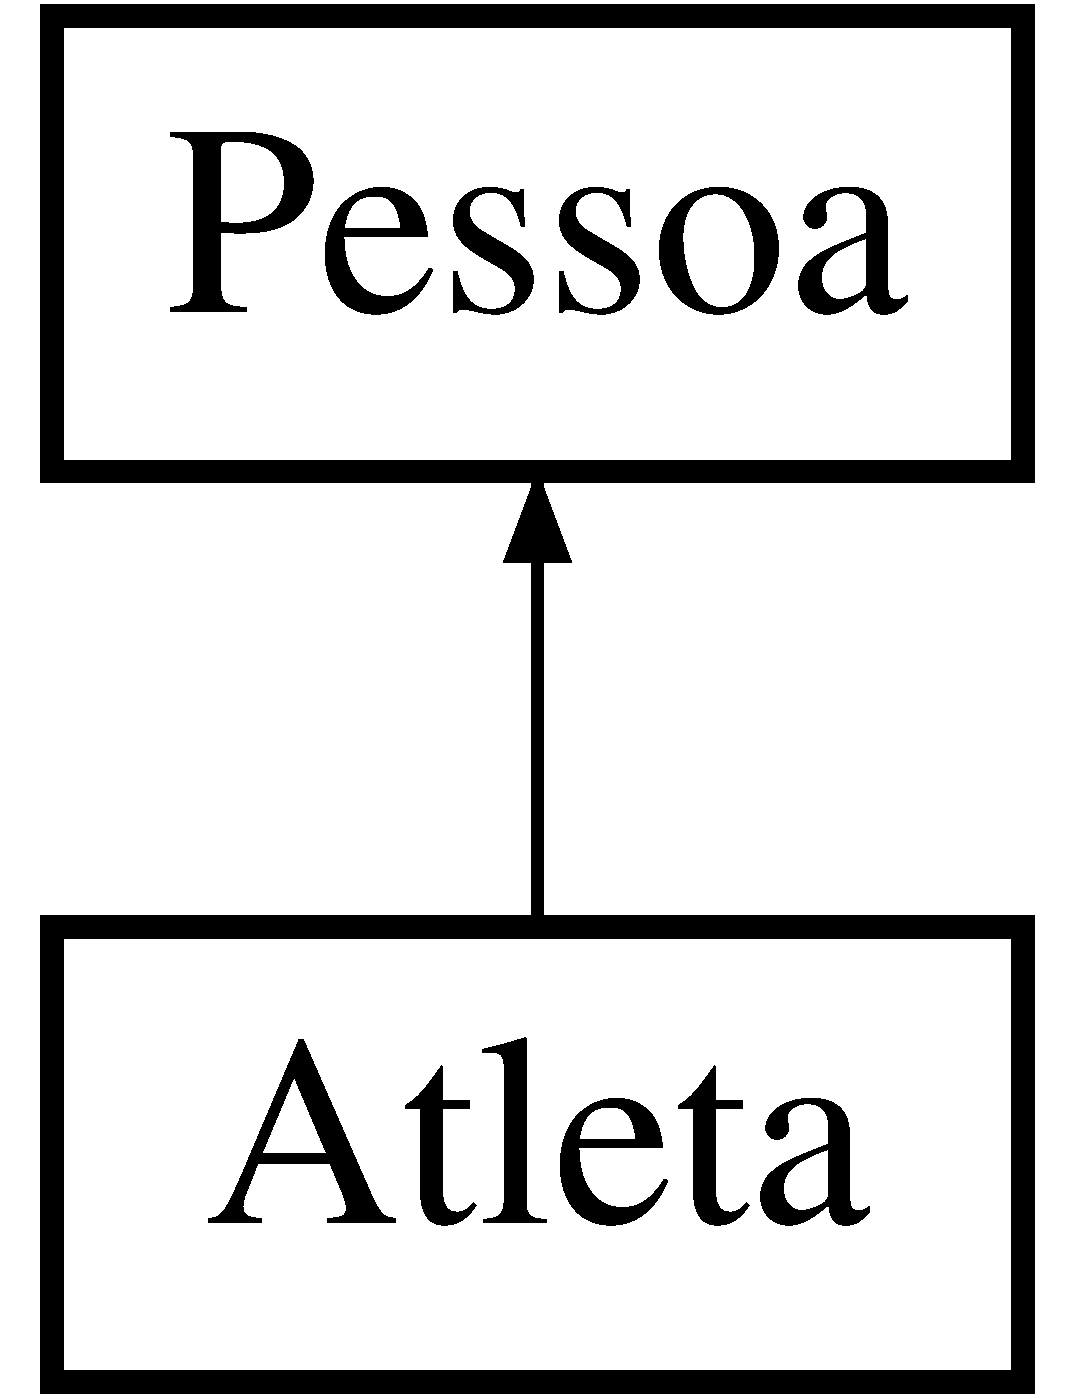
\includegraphics[height=2.000000cm]{class_atleta}
\end{center}
\end{figure}
\subsection*{Public Member Functions}
\begin{DoxyCompactItemize}
\item 
\hypertarget{class_atleta_afd38493a225fe3ae9cb23e2fe41e0297}{}{\bfseries Atleta} (string name, unsigned int age, float weight, float height)\label{class_atleta_afd38493a225fe3ae9cb23e2fe41e0297}

\item 
\hypertarget{class_atleta_a1bc03ab63e8621c634f782806180bdb8}{}float {\bfseries get\+Peso} () const \label{class_atleta_a1bc03ab63e8621c634f782806180bdb8}

\item 
\hypertarget{class_atleta_a2e801fd3feca11002de4cfd087621b5f}{}float {\bfseries get\+Estatura} () const \label{class_atleta_a2e801fd3feca11002de4cfd087621b5f}

\item 
\hypertarget{class_atleta_a8be582bd9aa951b768309f6bca996107}{}\hyperlink{class_equipa}{Equipa} $\ast$ {\bfseries get\+Equipa} ()\label{class_atleta_a8be582bd9aa951b768309f6bca996107}

\item 
\hypertarget{class_atleta_a4e77388fb86a570e76fb581115500cdb}{}void {\bfseries set\+Equipa} (\hyperlink{class_equipa}{Equipa} $\ast$equi)\label{class_atleta_a4e77388fb86a570e76fb581115500cdb}

\item 
\hypertarget{class_atleta_a9a7d709560b68c2cc05c8f9b0d27e864}{}void {\bfseries info} ()\label{class_atleta_a9a7d709560b68c2cc05c8f9b0d27e864}

\end{DoxyCompactItemize}


The documentation for this class was generated from the following files\+:\begin{DoxyCompactItemize}
\item 
src/Atleta.\+h\item 
src/Atleta.\+cpp\end{DoxyCompactItemize}

\hypertarget{class_atleta_inexistente}{}\section{Atleta\+Inexistente Class Reference}
\label{class_atleta_inexistente}\index{Atleta\+Inexistente@{Atleta\+Inexistente}}
Inheritance diagram for Atleta\+Inexistente\+:\begin{figure}[H]
\begin{center}
\leavevmode
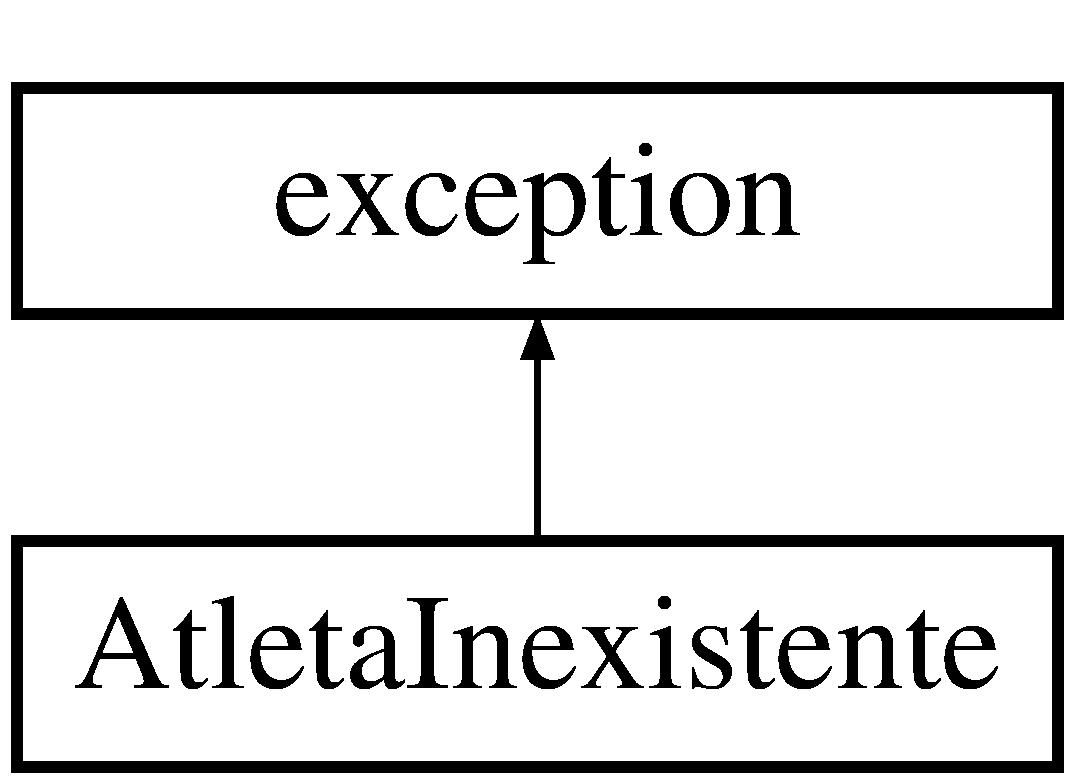
\includegraphics[height=2.000000cm]{class_atleta_inexistente}
\end{center}
\end{figure}
\subsection*{Public Member Functions}
\begin{DoxyCompactItemize}
\item 
\hypertarget{class_atleta_inexistente_aa1e33f37ed7f61ad74f6fdd6bb1d2d79}{}{\bfseries Atleta\+Inexistente} (string name\+Athlete)\label{class_atleta_inexistente_aa1e33f37ed7f61ad74f6fdd6bb1d2d79}

\item 
\hypertarget{class_atleta_inexistente_a845d43b61aab45329431d8cbf2f36f10}{}virtual const char $\ast$ {\bfseries what} () const   throw ()\label{class_atleta_inexistente_a845d43b61aab45329431d8cbf2f36f10}

\end{DoxyCompactItemize}


The documentation for this class was generated from the following file\+:\begin{DoxyCompactItemize}
\item 
src/Exceptions.\+h\end{DoxyCompactItemize}

\hypertarget{class_atleta_ja_existente}{}\section{Atleta\+Ja\+Existente Class Reference}
\label{class_atleta_ja_existente}\index{Atleta\+Ja\+Existente@{Atleta\+Ja\+Existente}}
Inheritance diagram for Atleta\+Ja\+Existente\+:\begin{figure}[H]
\begin{center}
\leavevmode
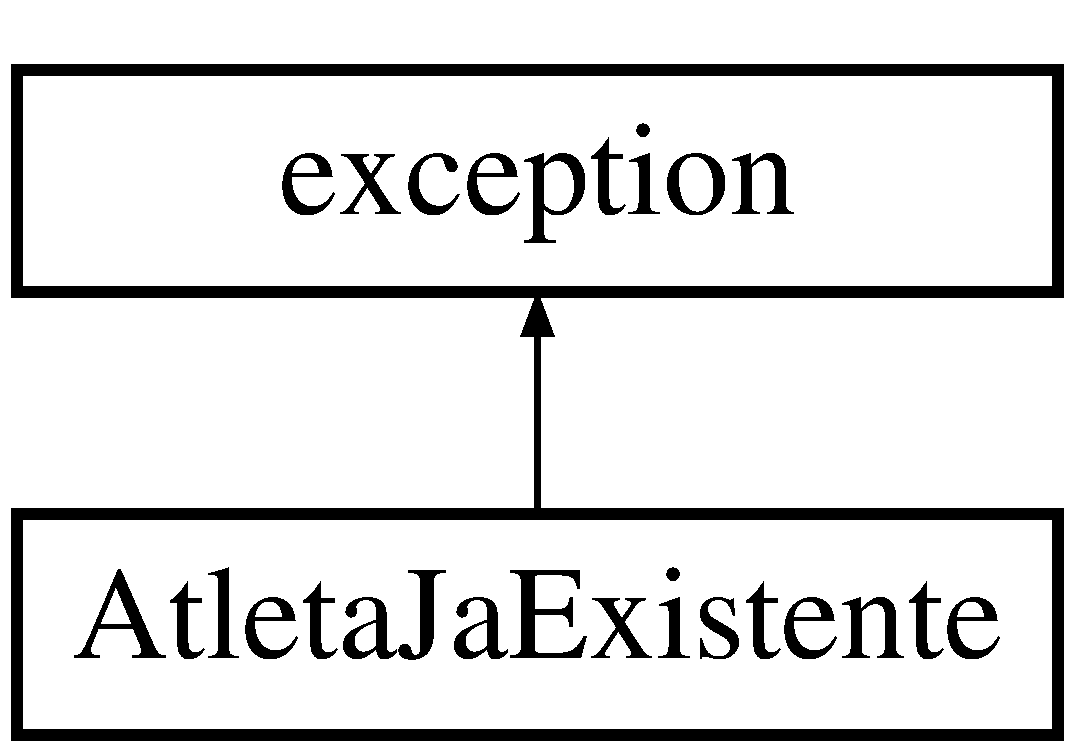
\includegraphics[height=2.000000cm]{class_atleta_ja_existente}
\end{center}
\end{figure}
\subsection*{Public Member Functions}
\begin{DoxyCompactItemize}
\item 
\hypertarget{class_atleta_ja_existente_ab51b6a99643cf6969b41fd94e3282775}{}{\bfseries Atleta\+Ja\+Existente} (string name\+Athlete)\label{class_atleta_ja_existente_ab51b6a99643cf6969b41fd94e3282775}

\item 
\hypertarget{class_atleta_ja_existente_a25c8a0dbbae34cced2758e0e3ca7c041}{}virtual const char $\ast$ {\bfseries what} () const   throw ()\label{class_atleta_ja_existente_a25c8a0dbbae34cced2758e0e3ca7c041}

\end{DoxyCompactItemize}


The documentation for this class was generated from the following file\+:\begin{DoxyCompactItemize}
\item 
src/Exceptions.\+h\end{DoxyCompactItemize}

\hypertarget{class_campeonato}{}\section{Campeonato Class Reference}
\label{class_campeonato}\index{Campeonato@{Campeonato}}
\subsection*{Public Member Functions}
\begin{DoxyCompactItemize}
\item 
\hypertarget{class_campeonato_a719acf7e9d7053578ac0be5ce87c2ea2}{}vector$<$ \hyperlink{class_equipa}{Equipa} $\ast$ $>$ {\bfseries get\+Equipas} ()\label{class_campeonato_a719acf7e9d7053578ac0be5ce87c2ea2}

\item 
\hypertarget{class_campeonato_ad86008ec57adfadd03b0e6982a4f02d6}{}vector$<$ \hyperlink{class_atleta}{Atleta} $\ast$ $>$ {\bfseries get\+Atletas} ()\label{class_campeonato_ad86008ec57adfadd03b0e6982a4f02d6}

\item 
\hypertarget{class_campeonato_a5c4288c01e533e165bbfc965bd768640}{}vector$<$ \hyperlink{class_modalidade}{Modalidade} $\ast$ $>$ {\bfseries get\+Modalidades} ()\label{class_campeonato_a5c4288c01e533e165bbfc965bd768640}

\item 
\hypertarget{class_campeonato_a0f77135234349b6547980a1e33b3048b}{}vector$<$ \hyperlink{class_prova}{Prova} $\ast$ $>$ {\bfseries get\+Provas} ()\label{class_campeonato_a0f77135234349b6547980a1e33b3048b}

\item 
\hypertarget{class_campeonato_a8e8c964209b423f187758ba2cdd80f67}{}vector$<$ \hyperlink{class_desporto}{Desporto} $\ast$ $>$ {\bfseries get\+Desportos} ()\label{class_campeonato_a8e8c964209b423f187758ba2cdd80f67}

\item 
\hypertarget{class_campeonato_a195c40661d8b3795c99a9b6bb1d590e5}{}vector$<$ \hyperlink{class_infrastrutura}{Infrastrutura} $\ast$ $>$ {\bfseries get\+Infrastruturas} ()\label{class_campeonato_a195c40661d8b3795c99a9b6bb1d590e5}

\item 
\hypertarget{class_campeonato_ab97078647cdfe861697fa1f940fd15cc}{}vector$<$ \hyperlink{class_funcionario}{Funcionario} $\ast$ $>$ {\bfseries get\+Funcionarios} ()\label{class_campeonato_ab97078647cdfe861697fa1f940fd15cc}

\item 
\hyperlink{class_equipa}{Equipa} $\ast$ \hyperlink{class_campeonato_a9cf172b084b661b4647f5010bddbcf34}{find\+Equipa} (string nome\+Equipa)
\item 
\hypertarget{class_campeonato_acde244f2b5f9124ef2842cb22f5dbc34}{}\hyperlink{class_atleta}{Atleta} $\ast$ {\bfseries find\+Atleta} (string nome\+Atleta)\label{class_campeonato_acde244f2b5f9124ef2842cb22f5dbc34}

\item 
\hypertarget{class_campeonato_a22d4d52592cbd305c2d7175f9402653b}{}\hyperlink{class_modalidade}{Modalidade} $\ast$ {\bfseries find\+Modalidade} (string nome\+Modalidade)\label{class_campeonato_a22d4d52592cbd305c2d7175f9402653b}

\item 
\hypertarget{class_campeonato_a0c7c6ba0950d1736a099bbc664df30c5}{}\hyperlink{class_prova}{Prova} $\ast$ {\bfseries find\+Prova} (string nome\+Prova)\label{class_campeonato_a0c7c6ba0950d1736a099bbc664df30c5}

\item 
\hypertarget{class_campeonato_af1301542ce4f7b1b77b52d0f69245031}{}\hyperlink{class_desporto}{Desporto} $\ast$ {\bfseries find\+Desporto} (string nome\+Desporto)\label{class_campeonato_af1301542ce4f7b1b77b52d0f69245031}

\item 
\hypertarget{class_campeonato_aff5ca14d9c636fbef9edd2db4ef8b371}{}\hyperlink{class_infrastrutura}{Infrastrutura} $\ast$ {\bfseries find\+Infrastrutura} (string nome\+Infrastrutura)\label{class_campeonato_aff5ca14d9c636fbef9edd2db4ef8b371}

\item 
\hypertarget{class_campeonato_a09706c3103fcb233036abce01a8b96c9}{}\hyperlink{class_funcionario}{Funcionario} $\ast$ {\bfseries find\+Funcionario} (string nome\+Funcionario)\label{class_campeonato_a09706c3103fcb233036abce01a8b96c9}

\item 
bool \hyperlink{class_campeonato_a7370b81eecbdb3c7fca8ca9400c039a9}{exists\+Equipa} (string nome\+Equipa)
\item 
\hypertarget{class_campeonato_a47f537905c392c2a0c58154164596ff3}{}bool {\bfseries exists\+Atleta} (string nome\+Atleta)\label{class_campeonato_a47f537905c392c2a0c58154164596ff3}

\item 
\hypertarget{class_campeonato_a4f97f51e378298db960324ecd323e0f4}{}bool {\bfseries exists\+Modalidade} (string nome\+Modalidade)\label{class_campeonato_a4f97f51e378298db960324ecd323e0f4}

\item 
\hypertarget{class_campeonato_ac246301cffebdadfc50c15b92fa73cbd}{}bool {\bfseries exists\+Prova} (string nome\+Prova)\label{class_campeonato_ac246301cffebdadfc50c15b92fa73cbd}

\item 
\hypertarget{class_campeonato_adfe05f4fe82ef6b27fb2f5107c85c3bf}{}bool {\bfseries exists\+Desporto} (string nome\+Desporto)\label{class_campeonato_adfe05f4fe82ef6b27fb2f5107c85c3bf}

\item 
\hypertarget{class_campeonato_ae69218519694b86b63da4118fdb3c563}{}bool {\bfseries exists\+Infrastrutura} (string nome\+Infrastrutura)\label{class_campeonato_ae69218519694b86b63da4118fdb3c563}

\item 
\hypertarget{class_campeonato_a532a52907e1e324168e4fc25c8f307fe}{}bool {\bfseries exists\+Funcionario} (string nome\+Funcionario)\label{class_campeonato_a532a52907e1e324168e4fc25c8f307fe}

\item 
\hypertarget{class_campeonato_a7f9818dfbb32ebfdff022b5194e1f268}{}bool {\bfseries Can\+Atleta\+Enter\+Modalidade} (string nome\+Modalidade, string nome\+Atleta)\label{class_campeonato_a7f9818dfbb32ebfdff022b5194e1f268}

\item 
void \hyperlink{class_campeonato_a80cf04fda33aa4f3d83d409e064aec01}{erase\+Atleta\+Modalidade} (string nome\+Modalidade, string nome\+Atleta)
\item 
\hypertarget{class_campeonato_a8e935d7b37d19565c317402d0a532a68}{}void {\bfseries erase\+Equipa} (string nome\+Equipa)\label{class_campeonato_a8e935d7b37d19565c317402d0a532a68}

\item 
\hypertarget{class_campeonato_acd7c3f6a223f822f66eab6af95602b8d}{}void {\bfseries erase\+Atleta} (string nome\+Atleta)\label{class_campeonato_acd7c3f6a223f822f66eab6af95602b8d}

\item 
\hypertarget{class_campeonato_a71bc500716b9fa2f65d5650625f94589}{}void {\bfseries erase\+Desporto} (string nome\+Desporto)\label{class_campeonato_a71bc500716b9fa2f65d5650625f94589}

\item 
\hypertarget{class_campeonato_acd4dd3e34af0e1cdc217c5a7d0233f9b}{}void {\bfseries erase\+Prova} (string nome\+Prova)\label{class_campeonato_acd4dd3e34af0e1cdc217c5a7d0233f9b}

\item 
\hypertarget{class_campeonato_ab9c05c50791fc841fa94ee9a5671e9cf}{}void {\bfseries erase\+Infrastrutura} (string nome\+Infrastrutura)\label{class_campeonato_ab9c05c50791fc841fa94ee9a5671e9cf}

\item 
\hypertarget{class_campeonato_abc621f4b26cbda73e700ae2bd757e52b}{}void {\bfseries erase\+Funcionario} (string nome\+Funcionario)\label{class_campeonato_abc621f4b26cbda73e700ae2bd757e52b}

\item 
void \hyperlink{class_campeonato_a9e16c686a4b5388978c9523da2d14393}{load\+Equipas} ()
\item 
\hypertarget{class_campeonato_a5d84a164e4acbd7c1c3eef304677754f}{}void {\bfseries save\+Equipa} ()\label{class_campeonato_a5d84a164e4acbd7c1c3eef304677754f}

\item 
\hypertarget{class_campeonato_a4a436d5b73072a16897b00f6781e749f}{}void {\bfseries add\+Equipa} (\hyperlink{class_equipa}{Equipa} $\ast$equi)\label{class_campeonato_a4a436d5b73072a16897b00f6781e749f}

\item 
\hypertarget{class_campeonato_afa2f81839bea9fa595861d7320210ab5}{}void {\bfseries load\+Atletas} ()\label{class_campeonato_afa2f81839bea9fa595861d7320210ab5}

\item 
\hypertarget{class_campeonato_adbbf4389d5aba7da1ed9b32acf89e6eb}{}void {\bfseries save\+Atleta} ()\label{class_campeonato_adbbf4389d5aba7da1ed9b32acf89e6eb}

\item 
\hypertarget{class_campeonato_a1897e31f57f82f54354e248514627732}{}void {\bfseries add\+Atleta} (\hyperlink{class_atleta}{Atleta} $\ast$atl)\label{class_campeonato_a1897e31f57f82f54354e248514627732}

\item 
\hypertarget{class_campeonato_aef8c4ac585a4fb31f36c79a446ea7e74}{}void {\bfseries load\+Modalidades} ()\label{class_campeonato_aef8c4ac585a4fb31f36c79a446ea7e74}

\item 
\hypertarget{class_campeonato_a9930be88df76b23b869f8b59225c33e6}{}void {\bfseries save\+Modalidade} ()\label{class_campeonato_a9930be88df76b23b869f8b59225c33e6}

\item 
\hypertarget{class_campeonato_ac3b0f8f58de8702ec16c0ad1f019aec2}{}void {\bfseries add\+Modalidade} (\hyperlink{class_modalidade}{Modalidade} $\ast$modal)\label{class_campeonato_ac3b0f8f58de8702ec16c0ad1f019aec2}

\item 
\hypertarget{class_campeonato_ab5e16dc2945f8d7c8df296f6ea9bcea7}{}void {\bfseries load\+Provas} ()\label{class_campeonato_ab5e16dc2945f8d7c8df296f6ea9bcea7}

\item 
\hypertarget{class_campeonato_a218d92de18b9b220152c45cf296c642a}{}void {\bfseries save\+Prova} ()\label{class_campeonato_a218d92de18b9b220152c45cf296c642a}

\item 
\hypertarget{class_campeonato_a777ce5868c70203d5f10957ee16ff809}{}void {\bfseries add\+Prova} (\hyperlink{class_prova}{Prova} $\ast$prova)\label{class_campeonato_a777ce5868c70203d5f10957ee16ff809}

\item 
\hypertarget{class_campeonato_a7f0315c9ea9ba62140421c60e5ff5e3b}{}void {\bfseries load\+Desportos} ()\label{class_campeonato_a7f0315c9ea9ba62140421c60e5ff5e3b}

\item 
\hypertarget{class_campeonato_a1bab4414a1ef07dc98870869e89ea958}{}void {\bfseries save\+Desporto} ()\label{class_campeonato_a1bab4414a1ef07dc98870869e89ea958}

\item 
\hypertarget{class_campeonato_a868d9ddabd78de968cd48a02b25c582f}{}void {\bfseries add\+Desporto} (\hyperlink{class_desporto}{Desporto} $\ast$desp)\label{class_campeonato_a868d9ddabd78de968cd48a02b25c582f}

\item 
\hypertarget{class_campeonato_ae3836a81c3eed0f733e4e755b90b698e}{}void {\bfseries load\+Infrastruturas} ()\label{class_campeonato_ae3836a81c3eed0f733e4e755b90b698e}

\item 
\hypertarget{class_campeonato_a6cdf7ddac2a131aa092874e5661452e6}{}void {\bfseries save\+Infrastrutura} ()\label{class_campeonato_a6cdf7ddac2a131aa092874e5661452e6}

\item 
\hypertarget{class_campeonato_adad466bb56cf2f764e8bd184653059a8}{}void {\bfseries add\+Infrastrutura} (\hyperlink{class_infrastrutura}{Infrastrutura} $\ast$infra)\label{class_campeonato_adad466bb56cf2f764e8bd184653059a8}

\item 
\hypertarget{class_campeonato_a4e08ac62e5c8a7839033d141f2d33af5}{}void {\bfseries load\+Funcionarios} ()\label{class_campeonato_a4e08ac62e5c8a7839033d141f2d33af5}

\item 
\hypertarget{class_campeonato_a512ae39e1ccd4f5ef1d63a5cbba70533}{}void {\bfseries save\+Funcionario} ()\label{class_campeonato_a512ae39e1ccd4f5ef1d63a5cbba70533}

\item 
\hypertarget{class_campeonato_a69850f368a571f1c4a3f41a8cdf9134d}{}void {\bfseries add\+Funcionario} (\hyperlink{class_funcionario}{Funcionario} $\ast$func)\label{class_campeonato_a69850f368a571f1c4a3f41a8cdf9134d}

\item 
int \hyperlink{class_campeonato_a66b8999b519c0d332454eb5aa8e52f58}{find\+Atleta\+Index} (string nome\+Atleta)
\item 
\hypertarget{class_campeonato_a22ef72d5e68e7ad752c1f50b7c75bed3}{}void {\bfseries change\+Equipa} (int index, \hyperlink{class_equipa}{Equipa} $\ast$equi)\label{class_campeonato_a22ef72d5e68e7ad752c1f50b7c75bed3}

\item 
int \hyperlink{class_campeonato_a9d4fafde7ccc993491653808073bfbe9}{find\+Prova\+Index} (string nome\+Prova)
\item 
\hypertarget{class_campeonato_a459af23f81e62238fda6c0fb2f5899c6}{}void {\bfseries change\+Infrastrutura} (int index, \hyperlink{class_infrastrutura}{Infrastrutura} $\ast$infra)\label{class_campeonato_a459af23f81e62238fda6c0fb2f5899c6}

\item 
int \hyperlink{class_campeonato_a621b57918dd641742b1bdb127d00ae9a}{find\+Modalidade\+Index} (string nome\+Modalidade)
\item 
\hypertarget{class_campeonato_aa36651ab3d9d5719544c87d73fb69f8d}{}void {\bfseries change\+Modalidade} (int index, \hyperlink{class_modalidade}{Modalidade} $\ast$mod)\label{class_campeonato_aa36651ab3d9d5719544c87d73fb69f8d}

\item 
\hypertarget{class_campeonato_a77820e96721d4a0dfcaef5dcdec2792c}{}void {\bfseries classifica} (string nome\+Modalidade, string nome\+Prova)\label{class_campeonato_a77820e96721d4a0dfcaef5dcdec2792c}

\item 
\hypertarget{class_campeonato_a16d66166b3addf4f1dc21772b49c8340}{}void {\bfseries saveclassifica} ()\label{class_campeonato_a16d66166b3addf4f1dc21772b49c8340}

\item 
\hypertarget{class_campeonato_af408d39d887fcab1bad83b7d003acdb3}{}void {\bfseries loadclassifica} ()\label{class_campeonato_af408d39d887fcab1bad83b7d003acdb3}

\item 
\hypertarget{class_campeonato_a6d18e304117b1109bb80fc9f96345130}{}void {\bfseries Atribui\+Infrastrutura} (string nome\+Modalidade, string nome\+Prova, string infrastrutura)\label{class_campeonato_a6d18e304117b1109bb80fc9f96345130}

\end{DoxyCompactItemize}


\subsection{Member Function Documentation}
\hypertarget{class_campeonato_a80cf04fda33aa4f3d83d409e064aec01}{}\index{Campeonato@{Campeonato}!erase\+Atleta\+Modalidade@{erase\+Atleta\+Modalidade}}
\index{erase\+Atleta\+Modalidade@{erase\+Atleta\+Modalidade}!Campeonato@{Campeonato}}
\subsubsection[{erase\+Atleta\+Modalidade(string nome\+Modalidade, string nome\+Atleta)}]{\setlength{\rightskip}{0pt plus 5cm}void Campeonato\+::erase\+Atleta\+Modalidade (
\begin{DoxyParamCaption}
\item[{string}]{nome\+Modalidade, }
\item[{string}]{nome\+Atleta}
\end{DoxyParamCaption}
)}\label{class_campeonato_a80cf04fda33aa4f3d83d409e064aec01}
M\+E\+T\+O\+D\+O\+S P\+A\+R\+A E\+L\+I\+M\+I\+N\+A\+R O\+B\+J\+E\+T\+O\+S C\+O\+M U\+M D\+E\+T\+E\+R\+M\+I\+N\+A\+D\+O N\+O\+M\+E D\+O\+S V\+E\+T\+O\+R\+E\+S \hypertarget{class_campeonato_a7370b81eecbdb3c7fca8ca9400c039a9}{}\index{Campeonato@{Campeonato}!exists\+Equipa@{exists\+Equipa}}
\index{exists\+Equipa@{exists\+Equipa}!Campeonato@{Campeonato}}
\subsubsection[{exists\+Equipa(string nome\+Equipa)}]{\setlength{\rightskip}{0pt plus 5cm}bool Campeonato\+::exists\+Equipa (
\begin{DoxyParamCaption}
\item[{string}]{nome\+Equipa}
\end{DoxyParamCaption}
)}\label{class_campeonato_a7370b81eecbdb3c7fca8ca9400c039a9}
M\+E\+T\+O\+D\+O\+S P\+A\+R\+A S\+A\+B\+E\+R S\+E U\+M O\+B\+J\+E\+T\+O C\+O\+M U\+M D\+E\+T\+E\+R\+M\+I\+N\+A\+D\+O N\+O\+M\+E E\+X\+I\+S\+T\+E \hypertarget{class_campeonato_a66b8999b519c0d332454eb5aa8e52f58}{}\index{Campeonato@{Campeonato}!find\+Atleta\+Index@{find\+Atleta\+Index}}
\index{find\+Atleta\+Index@{find\+Atleta\+Index}!Campeonato@{Campeonato}}
\subsubsection[{find\+Atleta\+Index(string nome\+Atleta)}]{\setlength{\rightskip}{0pt plus 5cm}int Campeonato\+::find\+Atleta\+Index (
\begin{DoxyParamCaption}
\item[{string}]{nome\+Atleta}
\end{DoxyParamCaption}
)}\label{class_campeonato_a66b8999b519c0d332454eb5aa8e52f58}
M\+E\+T\+O\+D\+O\+S P\+A\+R\+A M\+U\+D\+A\+R U\+M A\+T\+L\+E\+T\+A D\+E E\+Q\+U\+I\+P\+A \hypertarget{class_campeonato_a9cf172b084b661b4647f5010bddbcf34}{}\index{Campeonato@{Campeonato}!find\+Equipa@{find\+Equipa}}
\index{find\+Equipa@{find\+Equipa}!Campeonato@{Campeonato}}
\subsubsection[{find\+Equipa(string nome\+Equipa)}]{\setlength{\rightskip}{0pt plus 5cm}{\bf Equipa} $\ast$ Campeonato\+::find\+Equipa (
\begin{DoxyParamCaption}
\item[{string}]{nome\+Equipa}
\end{DoxyParamCaption}
)}\label{class_campeonato_a9cf172b084b661b4647f5010bddbcf34}
M\+E\+T\+O\+D\+O\+S D\+E P\+R\+O\+C\+U\+R\+A D\+E O\+B\+J\+E\+T\+O\+S C\+O\+M D\+E\+T\+E\+R\+M\+I\+N\+A\+D\+O N\+O\+M\+E N\+O\+S V\+E\+T\+O\+R\+E\+S \hypertarget{class_campeonato_a621b57918dd641742b1bdb127d00ae9a}{}\index{Campeonato@{Campeonato}!find\+Modalidade\+Index@{find\+Modalidade\+Index}}
\index{find\+Modalidade\+Index@{find\+Modalidade\+Index}!Campeonato@{Campeonato}}
\subsubsection[{find\+Modalidade\+Index(string nome\+Modalidade)}]{\setlength{\rightskip}{0pt plus 5cm}int Campeonato\+::find\+Modalidade\+Index (
\begin{DoxyParamCaption}
\item[{string}]{nome\+Modalidade}
\end{DoxyParamCaption}
)}\label{class_campeonato_a621b57918dd641742b1bdb127d00ae9a}
M\+E\+T\+O\+D\+O\+S P\+A\+R\+A A\+D\+I\+C\+I\+O\+N\+A\+R A\+T\+L\+E\+T\+A\+S A U\+M\+A M\+O\+D\+A\+L\+I\+D\+A\+D\+E \hypertarget{class_campeonato_a9d4fafde7ccc993491653808073bfbe9}{}\index{Campeonato@{Campeonato}!find\+Prova\+Index@{find\+Prova\+Index}}
\index{find\+Prova\+Index@{find\+Prova\+Index}!Campeonato@{Campeonato}}
\subsubsection[{find\+Prova\+Index(string nome\+Prova)}]{\setlength{\rightskip}{0pt plus 5cm}int Campeonato\+::find\+Prova\+Index (
\begin{DoxyParamCaption}
\item[{string}]{nome\+Prova}
\end{DoxyParamCaption}
)}\label{class_campeonato_a9d4fafde7ccc993491653808073bfbe9}
M\+E\+T\+O\+D\+O\+S P\+A\+R\+A M\+U\+D\+A\+R A I\+N\+F\+R\+A\+S\+T\+R\+U\+T\+U\+R\+A D\+E U\+M\+A P\+R\+O\+V\+A \hypertarget{class_campeonato_a9e16c686a4b5388978c9523da2d14393}{}\index{Campeonato@{Campeonato}!load\+Equipas@{load\+Equipas}}
\index{load\+Equipas@{load\+Equipas}!Campeonato@{Campeonato}}
\subsubsection[{load\+Equipas()}]{\setlength{\rightskip}{0pt plus 5cm}void Campeonato\+::load\+Equipas (
\begin{DoxyParamCaption}
{}
\end{DoxyParamCaption}
)}\label{class_campeonato_a9e16c686a4b5388978c9523da2d14393}
M\+E\+T\+O\+D\+O\+S D\+E S\+A\+V\+E/\+L\+O\+A\+D D\+O\+S V\+E\+T\+O\+R\+E\+S E F\+I\+C\+H\+E\+I\+R\+O\+S 

The documentation for this class was generated from the following files\+:\begin{DoxyCompactItemize}
\item 
src/Campeonato.\+h\item 
src/Campeonato.\+cpp\end{DoxyCompactItemize}

\hypertarget{class_desporto}{}\section{Desporto Class Reference}
\label{class_desporto}\index{Desporto@{Desporto}}
\subsection*{Public Member Functions}
\begin{DoxyCompactItemize}
\item 
\hypertarget{class_desporto_a5d74506380974d05a2d79c21527ffc83}{}{\bfseries Desporto} (string name)\label{class_desporto_a5d74506380974d05a2d79c21527ffc83}

\item 
\hypertarget{class_desporto_ab8a8413f056aeaa6dbd55730a7b6cd85}{}string {\bfseries get\+Nome} () const \label{class_desporto_ab8a8413f056aeaa6dbd55730a7b6cd85}

\item 
\hypertarget{class_desporto_af8436b5a0694a82b3105d2b81cea9166}{}vector$<$ \hyperlink{class_modalidade}{Modalidade} $\ast$ $>$ {\bfseries get\+Modalidades} ()\label{class_desporto_af8436b5a0694a82b3105d2b81cea9166}

\item 
\hypertarget{class_desporto_a67b1e45c5dc36c7b5d34a96b53e3fe32}{}void {\bfseries push\+Modalidade} (\hyperlink{class_modalidade}{Modalidade} $\ast$modal)\label{class_desporto_a67b1e45c5dc36c7b5d34a96b53e3fe32}

\end{DoxyCompactItemize}


The documentation for this class was generated from the following files\+:\begin{DoxyCompactItemize}
\item 
src/Desporto.\+h\item 
src/Desporto.\+cpp\end{DoxyCompactItemize}

\hypertarget{class_desporto_inexistente}{}\section{Desporto\+Inexistente Class Reference}
\label{class_desporto_inexistente}\index{Desporto\+Inexistente@{Desporto\+Inexistente}}
Inheritance diagram for Desporto\+Inexistente\+:\begin{figure}[H]
\begin{center}
\leavevmode
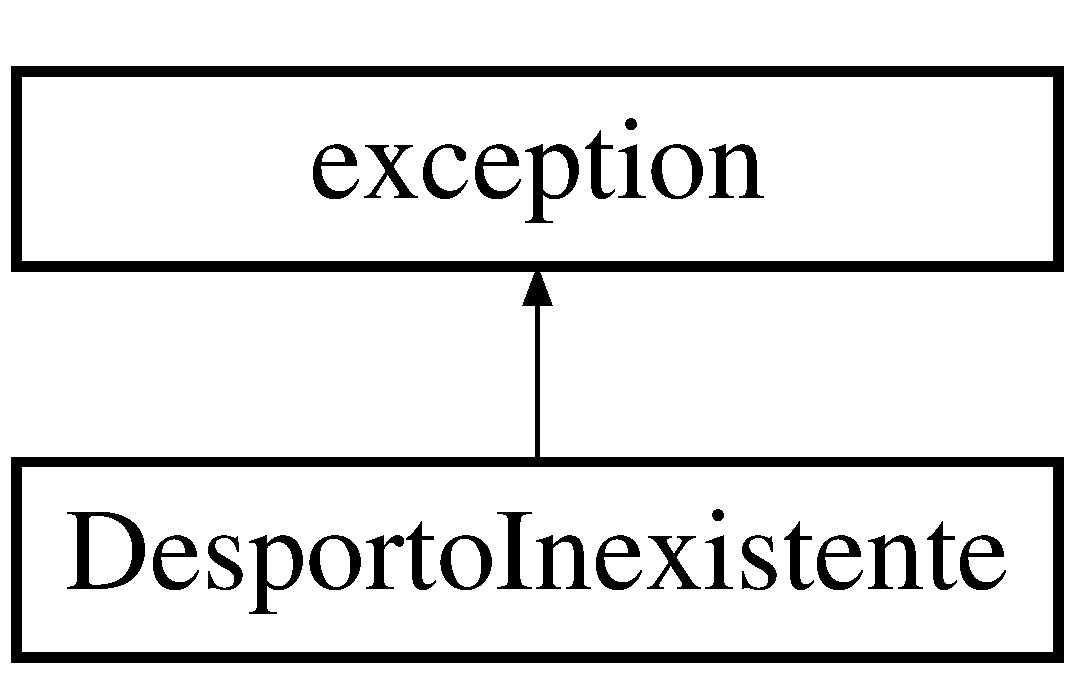
\includegraphics[height=2.000000cm]{class_desporto_inexistente}
\end{center}
\end{figure}
\subsection*{Public Member Functions}
\begin{DoxyCompactItemize}
\item 
\hypertarget{class_desporto_inexistente_a4fb6dfe8d0367a974ab2772c57d871aa}{}{\bfseries Desporto\+Inexistente} (string name\+Sport)\label{class_desporto_inexistente_a4fb6dfe8d0367a974ab2772c57d871aa}

\item 
\hypertarget{class_desporto_inexistente_a3e8b2e51b61fd50b55e0854199e348c7}{}virtual const char $\ast$ {\bfseries what} () const   throw ()\label{class_desporto_inexistente_a3e8b2e51b61fd50b55e0854199e348c7}

\end{DoxyCompactItemize}


The documentation for this class was generated from the following file\+:\begin{DoxyCompactItemize}
\item 
src/Exceptions.\+h\end{DoxyCompactItemize}

\hypertarget{class_desporto_ja_existente}{}\section{Desporto\+Ja\+Existente Class Reference}
\label{class_desporto_ja_existente}\index{Desporto\+Ja\+Existente@{Desporto\+Ja\+Existente}}
Inheritance diagram for Desporto\+Ja\+Existente\+:\begin{figure}[H]
\begin{center}
\leavevmode
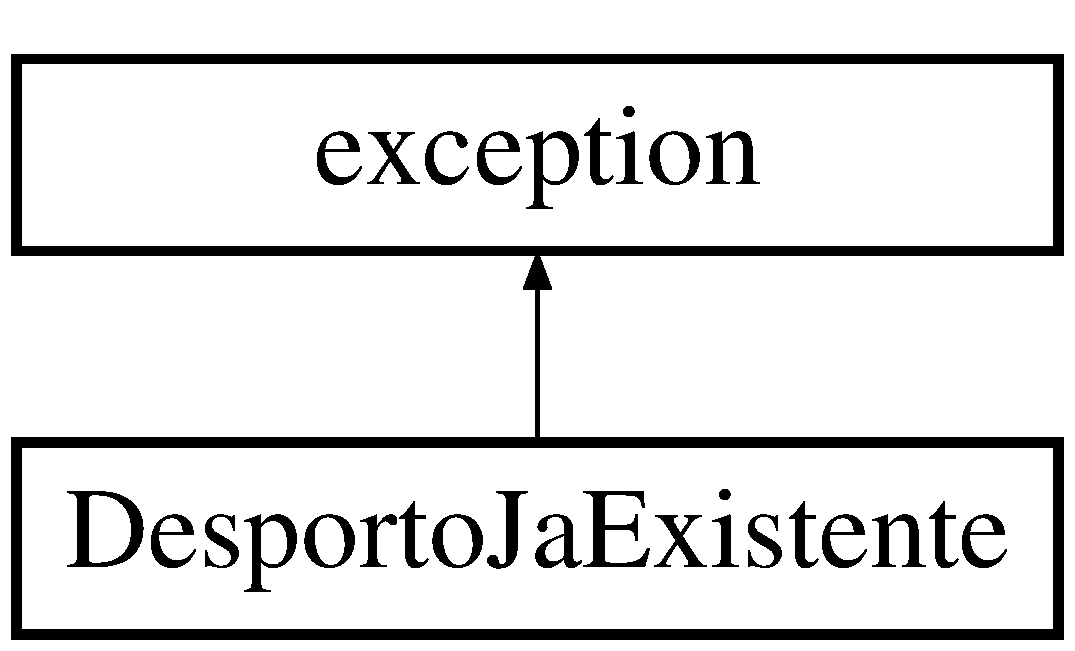
\includegraphics[height=2.000000cm]{class_desporto_ja_existente}
\end{center}
\end{figure}
\subsection*{Public Member Functions}
\begin{DoxyCompactItemize}
\item 
\hypertarget{class_desporto_ja_existente_a915af6fa35b053a6e69c92e5812f4c9d}{}{\bfseries Desporto\+Ja\+Existente} (string name\+Sport)\label{class_desporto_ja_existente_a915af6fa35b053a6e69c92e5812f4c9d}

\item 
\hypertarget{class_desporto_ja_existente_ac65f5fc9efc431f555d4153fb546475f}{}virtual const char $\ast$ {\bfseries what} () const   throw ()\label{class_desporto_ja_existente_ac65f5fc9efc431f555d4153fb546475f}

\end{DoxyCompactItemize}


The documentation for this class was generated from the following file\+:\begin{DoxyCompactItemize}
\item 
src/Exceptions.\+h\end{DoxyCompactItemize}

\hypertarget{class_equipa}{}\section{Equipa Class Reference}
\label{class_equipa}\index{Equipa@{Equipa}}
\subsection*{Public Member Functions}
\begin{DoxyCompactItemize}
\item 
\hypertarget{class_equipa_aff6ca66d2a63c796afdb807622876235}{}{\bfseries Equipa} (string name)\label{class_equipa_aff6ca66d2a63c796afdb807622876235}

\item 
\hypertarget{class_equipa_a9d20d0c8daa94e7562c5ea173337a224}{}string {\bfseries get\+Nome} () const \label{class_equipa_a9d20d0c8daa94e7562c5ea173337a224}

\item 
\hypertarget{class_equipa_a478806e57983511d7b44f4f69f80d28a}{}vector$<$ string $>$ {\bfseries get\+Desportos} ()\label{class_equipa_a478806e57983511d7b44f4f69f80d28a}

\item 
\hypertarget{class_equipa_a91e981a8a48f41460d14969d25142706}{}void {\bfseries push\+Desporto} (string desp)\label{class_equipa_a91e981a8a48f41460d14969d25142706}

\end{DoxyCompactItemize}


The documentation for this class was generated from the following files\+:\begin{DoxyCompactItemize}
\item 
src/Equipa.\+h\item 
src/Equipa.\+cpp\end{DoxyCompactItemize}

\hypertarget{class_equipa_inexistente}{}\section{Equipa\+Inexistente Class Reference}
\label{class_equipa_inexistente}\index{Equipa\+Inexistente@{Equipa\+Inexistente}}


{\ttfamily \#include $<$Exceptions.\+h$>$}

Inheritance diagram for Equipa\+Inexistente\+:\begin{figure}[H]
\begin{center}
\leavevmode
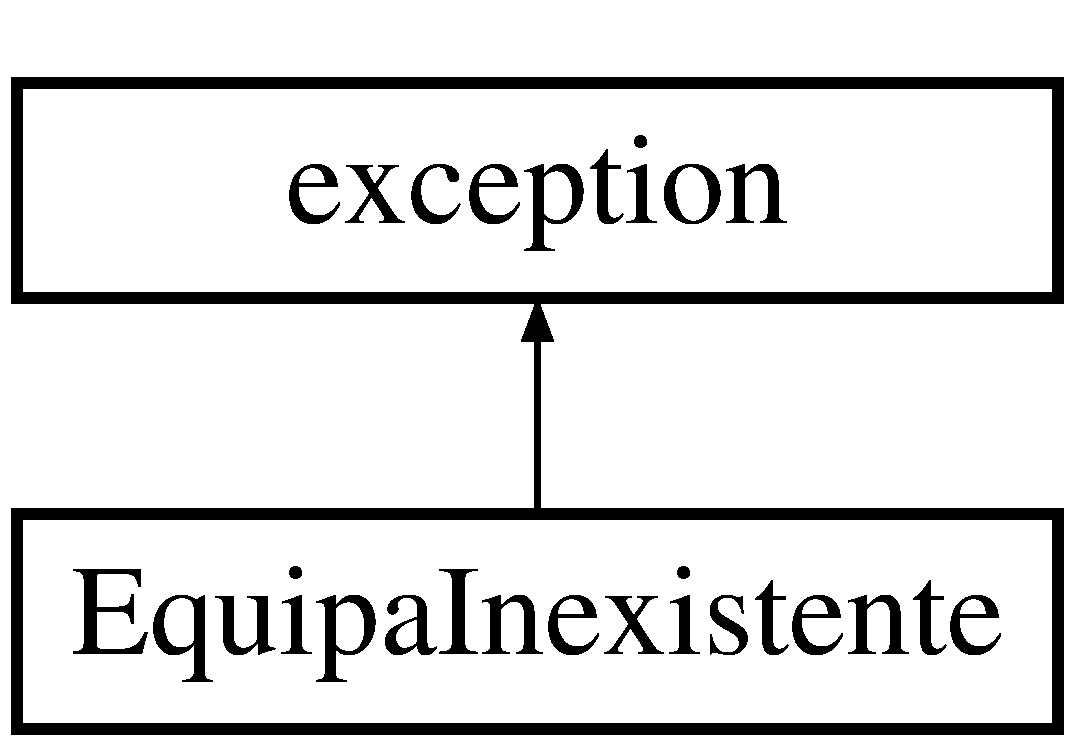
\includegraphics[height=2.000000cm]{class_equipa_inexistente}
\end{center}
\end{figure}
\subsection*{Public Member Functions}
\begin{DoxyCompactItemize}
\item 
\hypertarget{class_equipa_inexistente_a72e86bce0a8ae704277c59b9f36ab684}{}{\bfseries Equipa\+Inexistente} (string name\+Team)\label{class_equipa_inexistente_a72e86bce0a8ae704277c59b9f36ab684}

\item 
\hypertarget{class_equipa_inexistente_a6ad47a632d3ad739c8e4ebf71a9c5f5b}{}virtual const char $\ast$ {\bfseries what} () const   throw ()\label{class_equipa_inexistente_a6ad47a632d3ad739c8e4ebf71a9c5f5b}

\end{DoxyCompactItemize}


\subsection{Detailed Description}
E\+X\+C\+E�\+O\+E\+S I\+N\+E\+X\+I\+S\+T\+E\+N\+T\+E 

The documentation for this class was generated from the following file\+:\begin{DoxyCompactItemize}
\item 
src/Exceptions.\+h\end{DoxyCompactItemize}

\hypertarget{class_equipa_ja_existente}{}\section{Equipa\+Ja\+Existente Class Reference}
\label{class_equipa_ja_existente}\index{Equipa\+Ja\+Existente@{Equipa\+Ja\+Existente}}


{\ttfamily \#include $<$Exceptions.\+h$>$}

Inheritance diagram for Equipa\+Ja\+Existente\+:\begin{figure}[H]
\begin{center}
\leavevmode
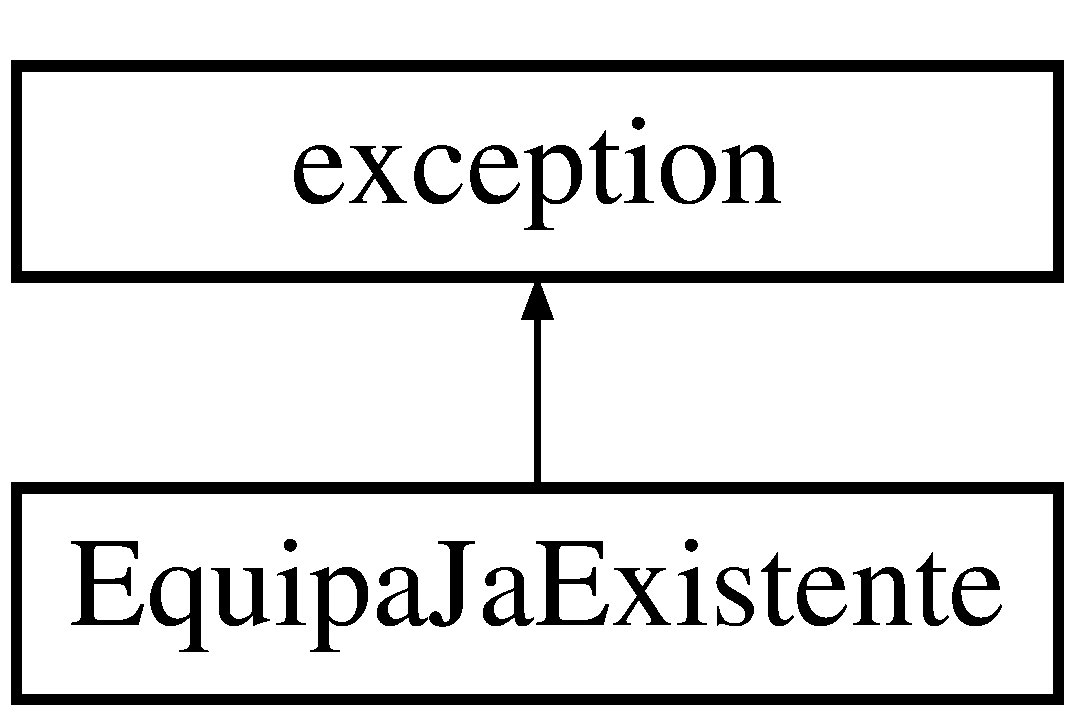
\includegraphics[height=2.000000cm]{class_equipa_ja_existente}
\end{center}
\end{figure}
\subsection*{Public Member Functions}
\begin{DoxyCompactItemize}
\item 
\hypertarget{class_equipa_ja_existente_a762d6487a95ee54204352126842993ec}{}{\bfseries Equipa\+Ja\+Existente} (string name\+Team)\label{class_equipa_ja_existente_a762d6487a95ee54204352126842993ec}

\item 
\hypertarget{class_equipa_ja_existente_adcafbb6bf19fd1a57d44f5a6bb628f2a}{}virtual const char $\ast$ {\bfseries what} () const   throw ()\label{class_equipa_ja_existente_adcafbb6bf19fd1a57d44f5a6bb628f2a}

\end{DoxyCompactItemize}


\subsection{Detailed Description}
E\+X\+C\+E��\+E\+S J�\+E\+X\+I\+S\+T\+E\+N\+T\+E 

The documentation for this class was generated from the following file\+:\begin{DoxyCompactItemize}
\item 
src/Exceptions.\+h\end{DoxyCompactItemize}

\hypertarget{class_funcionario}{}\section{Funcionario Class Reference}
\label{class_funcionario}\index{Funcionario@{Funcionario}}
Inheritance diagram for Funcionario\+:\begin{figure}[H]
\begin{center}
\leavevmode
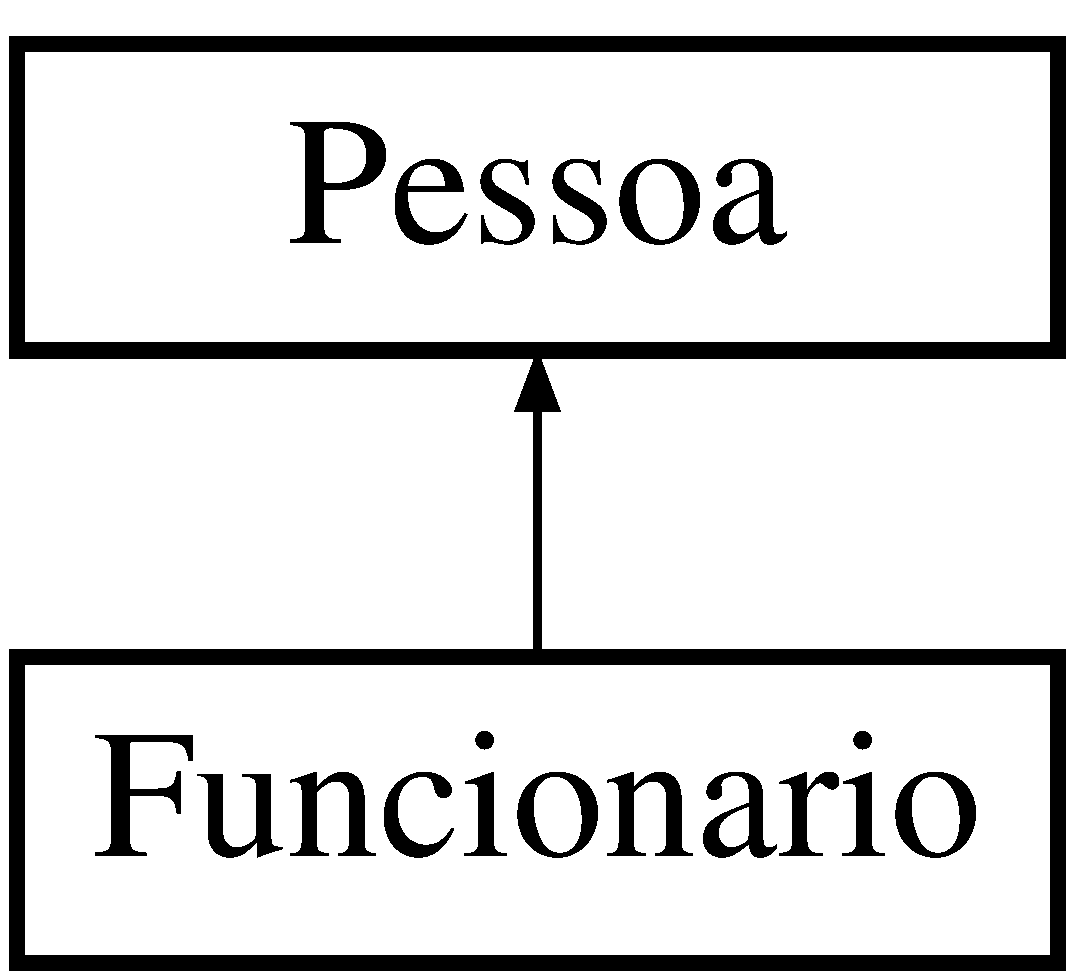
\includegraphics[height=2.000000cm]{class_funcionario}
\end{center}
\end{figure}
\subsection*{Public Member Functions}
\begin{DoxyCompactItemize}
\item 
\hypertarget{class_funcionario_affa57075f3e127d0d130e447e556207d}{}{\bfseries Funcionario} (string name, unsigned int age, int work\+\_\+years)\label{class_funcionario_affa57075f3e127d0d130e447e556207d}

\item 
\hypertarget{class_funcionario_a45068128fc425fda098cb113c0261693}{}int {\bfseries get\+Anos\+Trabalho} () const \label{class_funcionario_a45068128fc425fda098cb113c0261693}

\item 
\hypertarget{class_funcionario_a10fd5433afc1c2ef2061cf572429cb26}{}void {\bfseries info} ()\label{class_funcionario_a10fd5433afc1c2ef2061cf572429cb26}

\end{DoxyCompactItemize}


The documentation for this class was generated from the following files\+:\begin{DoxyCompactItemize}
\item 
src/Funcionario.\+h\item 
src/Funcionario.\+cpp\end{DoxyCompactItemize}

\hypertarget{class_funcionario_inexistente}{}\section{Funcionario\+Inexistente Class Reference}
\label{class_funcionario_inexistente}\index{Funcionario\+Inexistente@{Funcionario\+Inexistente}}
Inheritance diagram for Funcionario\+Inexistente\+:\begin{figure}[H]
\begin{center}
\leavevmode
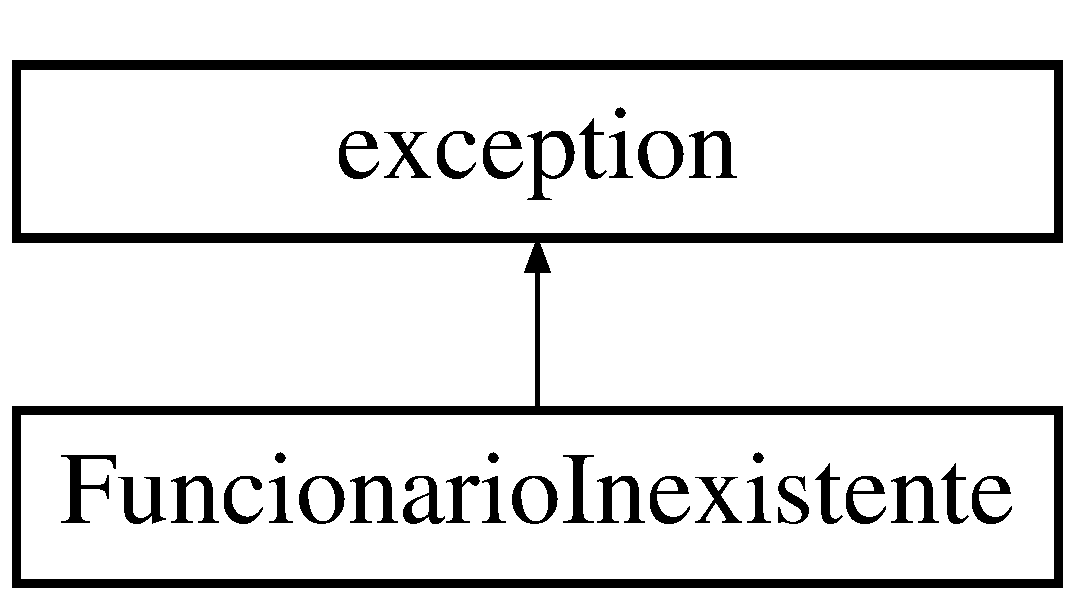
\includegraphics[height=2.000000cm]{class_funcionario_inexistente}
\end{center}
\end{figure}
\subsection*{Public Member Functions}
\begin{DoxyCompactItemize}
\item 
\hypertarget{class_funcionario_inexistente_a9efc9a1af26f64b0167a3ef37dbd95fb}{}{\bfseries Funcionario\+Inexistente} (string name\+Worker)\label{class_funcionario_inexistente_a9efc9a1af26f64b0167a3ef37dbd95fb}

\item 
\hypertarget{class_funcionario_inexistente_ae49d5868c8871518c5404a79d360892d}{}virtual const char $\ast$ {\bfseries what} () const   throw ()\label{class_funcionario_inexistente_ae49d5868c8871518c5404a79d360892d}

\end{DoxyCompactItemize}


The documentation for this class was generated from the following file\+:\begin{DoxyCompactItemize}
\item 
src/Exceptions.\+h\end{DoxyCompactItemize}

\hypertarget{class_funcionario_ja_existente}{}\section{Funcionario\+Ja\+Existente Class Reference}
\label{class_funcionario_ja_existente}\index{Funcionario\+Ja\+Existente@{Funcionario\+Ja\+Existente}}
Inheritance diagram for Funcionario\+Ja\+Existente\+:\begin{figure}[H]
\begin{center}
\leavevmode
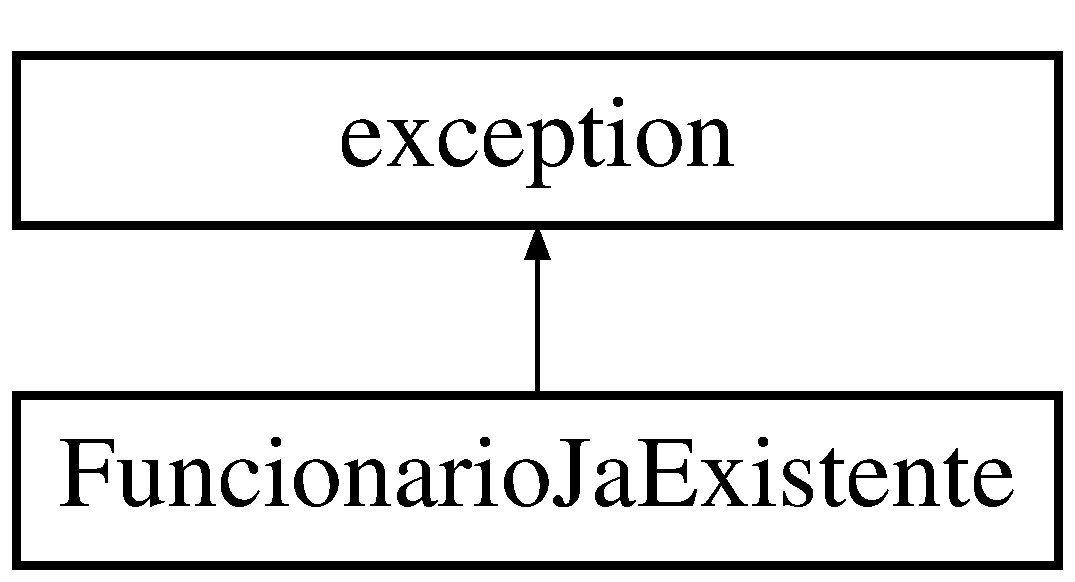
\includegraphics[height=2.000000cm]{class_funcionario_ja_existente}
\end{center}
\end{figure}
\subsection*{Public Member Functions}
\begin{DoxyCompactItemize}
\item 
\hypertarget{class_funcionario_ja_existente_ab9cbab1b79c5d63e996347be33521c41}{}{\bfseries Funcionario\+Ja\+Existente} (string name\+Worker)\label{class_funcionario_ja_existente_ab9cbab1b79c5d63e996347be33521c41}

\item 
\hypertarget{class_funcionario_ja_existente_a4a952853cf5e806fac06b7b08ed623f5}{}virtual const char $\ast$ {\bfseries what} () const   throw ()\label{class_funcionario_ja_existente_a4a952853cf5e806fac06b7b08ed623f5}

\end{DoxyCompactItemize}


The documentation for this class was generated from the following file\+:\begin{DoxyCompactItemize}
\item 
src/Exceptions.\+h\end{DoxyCompactItemize}

\hypertarget{class_idade_invalida}{}\section{Idade\+Invalida Class Reference}
\label{class_idade_invalida}\index{Idade\+Invalida@{Idade\+Invalida}}
Inheritance diagram for Idade\+Invalida\+:\begin{figure}[H]
\begin{center}
\leavevmode
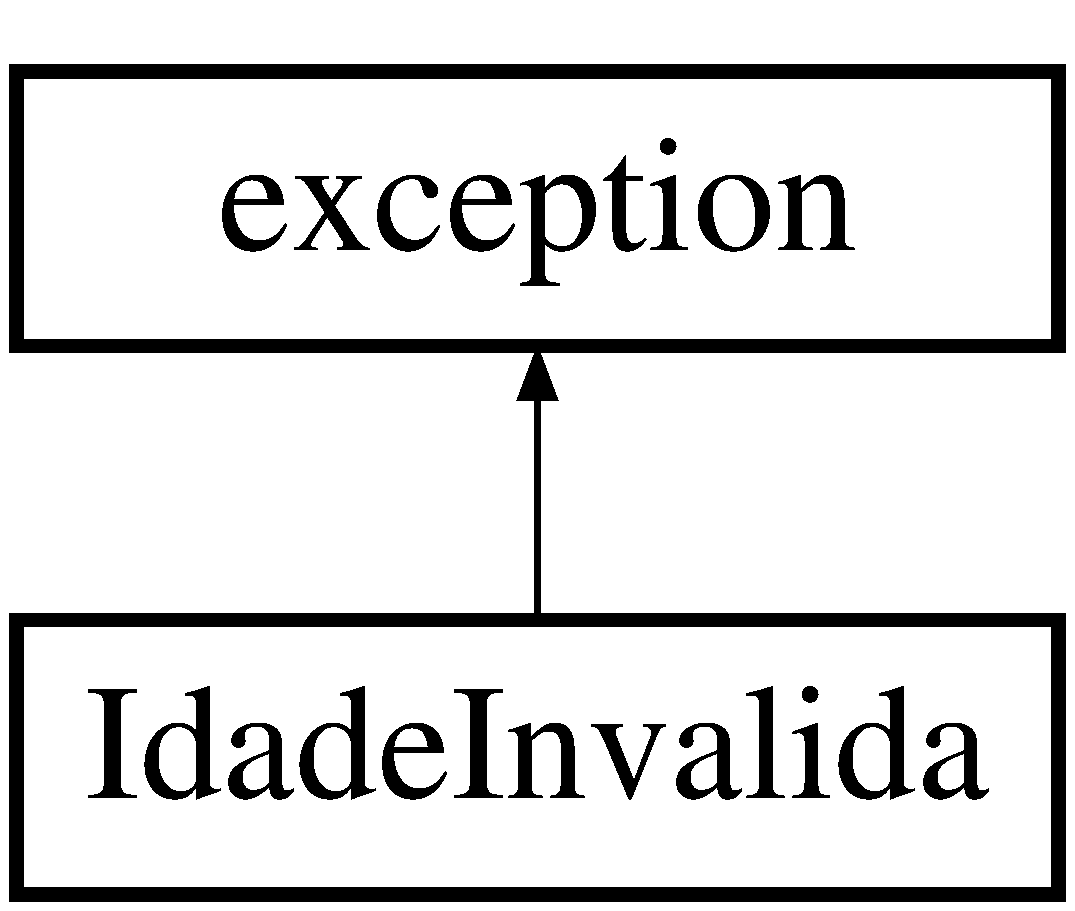
\includegraphics[height=2.000000cm]{class_idade_invalida}
\end{center}
\end{figure}
\subsection*{Public Member Functions}
\begin{DoxyCompactItemize}
\item 
\hypertarget{class_idade_invalida_aeac23b63d8109676c4597db7ee2487e9}{}virtual const char $\ast$ {\bfseries what} () const   throw ()\label{class_idade_invalida_aeac23b63d8109676c4597db7ee2487e9}

\end{DoxyCompactItemize}


The documentation for this class was generated from the following file\+:\begin{DoxyCompactItemize}
\item 
src/Exceptions.\+h\end{DoxyCompactItemize}

\hypertarget{class_infrastrutura}{}\section{Infrastrutura Class Reference}
\label{class_infrastrutura}\index{Infrastrutura@{Infrastrutura}}
\subsection*{Public Member Functions}
\begin{DoxyCompactItemize}
\item 
\hypertarget{class_infrastrutura_ac78bcb26b52106b69978b2f57221955a}{}{\bfseries Infrastrutura} (string name, string city)\label{class_infrastrutura_ac78bcb26b52106b69978b2f57221955a}

\item 
\hypertarget{class_infrastrutura_a14ba5d30c8ce9260d39be1dc7f2bb8c6}{}string {\bfseries get\+Nome} () const \label{class_infrastrutura_a14ba5d30c8ce9260d39be1dc7f2bb8c6}

\item 
\hypertarget{class_infrastrutura_af7dd3df24da0b2bf6a97d124fbfdc09c}{}string {\bfseries get\+Cidade} () const \label{class_infrastrutura_af7dd3df24da0b2bf6a97d124fbfdc09c}

\end{DoxyCompactItemize}


The documentation for this class was generated from the following files\+:\begin{DoxyCompactItemize}
\item 
src/Infrastrutura.\+h\item 
src/Infrastrutura.\+cpp\end{DoxyCompactItemize}

\hypertarget{class_infrastrutura_inexistente}{}\section{Infrastrutura\+Inexistente Class Reference}
\label{class_infrastrutura_inexistente}\index{Infrastrutura\+Inexistente@{Infrastrutura\+Inexistente}}
Inheritance diagram for Infrastrutura\+Inexistente\+:\begin{figure}[H]
\begin{center}
\leavevmode
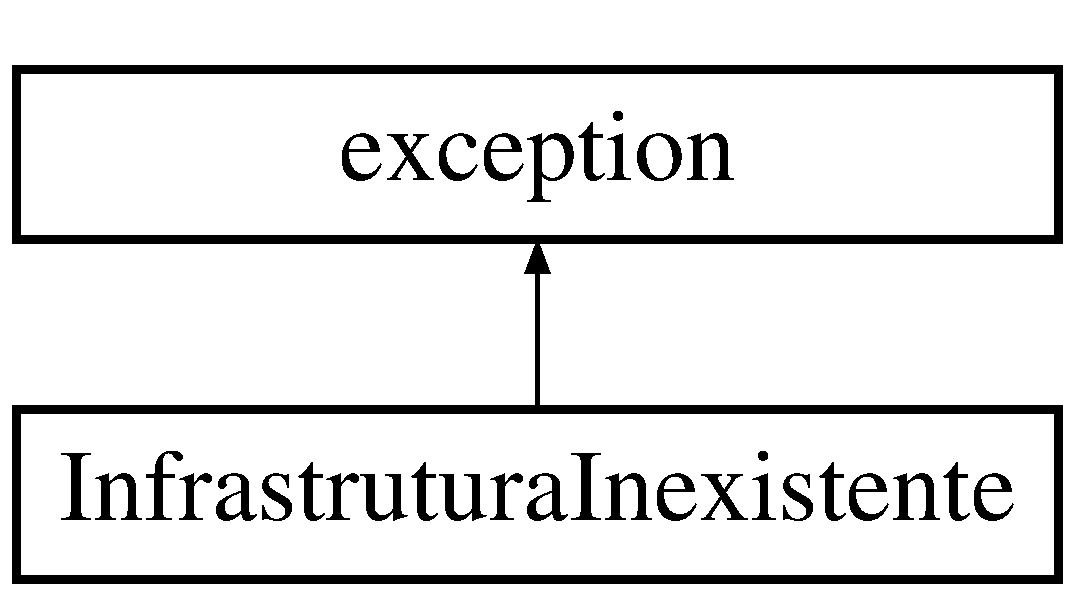
\includegraphics[height=2.000000cm]{class_infrastrutura_inexistente}
\end{center}
\end{figure}
\subsection*{Public Member Functions}
\begin{DoxyCompactItemize}
\item 
\hypertarget{class_infrastrutura_inexistente_ac177b75a9173440c1d939f4af85f2596}{}{\bfseries Infrastrutura\+Inexistente} (string name\+Infrastructure)\label{class_infrastrutura_inexistente_ac177b75a9173440c1d939f4af85f2596}

\item 
\hypertarget{class_infrastrutura_inexistente_aea5656e77e715c0f5634d34adf909142}{}virtual const char $\ast$ {\bfseries what} () const   throw ()\label{class_infrastrutura_inexistente_aea5656e77e715c0f5634d34adf909142}

\end{DoxyCompactItemize}


The documentation for this class was generated from the following file\+:\begin{DoxyCompactItemize}
\item 
src/Exceptions.\+h\end{DoxyCompactItemize}

\hypertarget{class_infrastrutura_ja_existente}{}\section{Infrastrutura\+Ja\+Existente Class Reference}
\label{class_infrastrutura_ja_existente}\index{Infrastrutura\+Ja\+Existente@{Infrastrutura\+Ja\+Existente}}
Inheritance diagram for Infrastrutura\+Ja\+Existente\+:\begin{figure}[H]
\begin{center}
\leavevmode
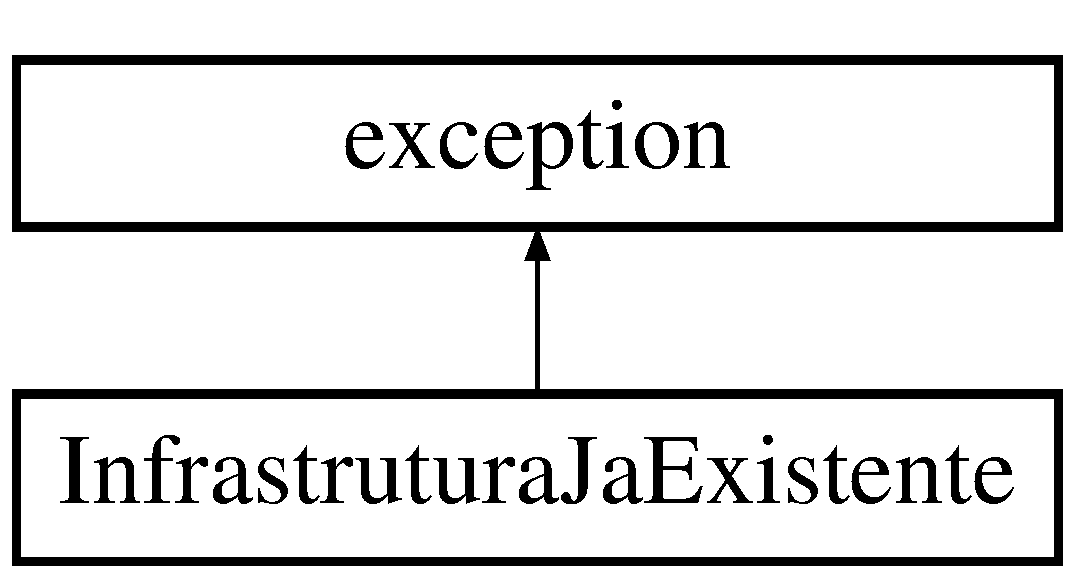
\includegraphics[height=2.000000cm]{class_infrastrutura_ja_existente}
\end{center}
\end{figure}
\subsection*{Public Member Functions}
\begin{DoxyCompactItemize}
\item 
\hypertarget{class_infrastrutura_ja_existente_aad900d6748672e39d934533d3734d6b9}{}{\bfseries Infrastrutura\+Ja\+Existente} (string name\+Infrastructure)\label{class_infrastrutura_ja_existente_aad900d6748672e39d934533d3734d6b9}

\item 
\hypertarget{class_infrastrutura_ja_existente_adbce6cb377f4d2b2ee5c0437ff489ebe}{}virtual const char $\ast$ {\bfseries what} () const   throw ()\label{class_infrastrutura_ja_existente_adbce6cb377f4d2b2ee5c0437ff489ebe}

\end{DoxyCompactItemize}


The documentation for this class was generated from the following file\+:\begin{DoxyCompactItemize}
\item 
src/Exceptions.\+h\end{DoxyCompactItemize}

\hypertarget{class_modalidade}{}\section{Modalidade Class Reference}
\label{class_modalidade}\index{Modalidade@{Modalidade}}
\subsection*{Public Member Functions}
\begin{DoxyCompactItemize}
\item 
\hypertarget{class_modalidade_aceeb2517503ed5dcb712890b280b9194}{}{\bfseries Modalidade} (string name)\label{class_modalidade_aceeb2517503ed5dcb712890b280b9194}

\item 
\hypertarget{class_modalidade_a46003f6a0dceac894f92971a6df9e4a7}{}string {\bfseries get\+Nome} () const \label{class_modalidade_a46003f6a0dceac894f92971a6df9e4a7}

\item 
\hypertarget{class_modalidade_a259ad3d7e3ba08a6167a632d1e216554}{}vector$<$ \hyperlink{class_atleta}{Atleta} $\ast$ $>$ {\bfseries get\+Atletas} ()\label{class_modalidade_a259ad3d7e3ba08a6167a632d1e216554}

\item 
\hypertarget{class_modalidade_ab1db62f8b54f8cec37ea2aa1ed2711a1}{}void {\bfseries push\+Atleta} (\hyperlink{class_atleta}{Atleta} $\ast$atl)\label{class_modalidade_ab1db62f8b54f8cec37ea2aa1ed2711a1}

\item 
\hypertarget{class_modalidade_ab93a5e17e9b85eb496ce7c82229e879a}{}void {\bfseries erase\+Atleta} (int index)\label{class_modalidade_ab93a5e17e9b85eb496ce7c82229e879a}

\item 
\hypertarget{class_modalidade_a39da8a6a7ed0009f6f2965db0001d85d}{}void {\bfseries erase\+Atleta2} (int index)\label{class_modalidade_a39da8a6a7ed0009f6f2965db0001d85d}

\end{DoxyCompactItemize}


The documentation for this class was generated from the following files\+:\begin{DoxyCompactItemize}
\item 
src/Modalidade.\+h\item 
src/Modalidade.\+cpp\end{DoxyCompactItemize}

\hypertarget{class_modalidade_inexistente}{}\section{Modalidade\+Inexistente Class Reference}
\label{class_modalidade_inexistente}\index{Modalidade\+Inexistente@{Modalidade\+Inexistente}}
Inheritance diagram for Modalidade\+Inexistente\+:\begin{figure}[H]
\begin{center}
\leavevmode
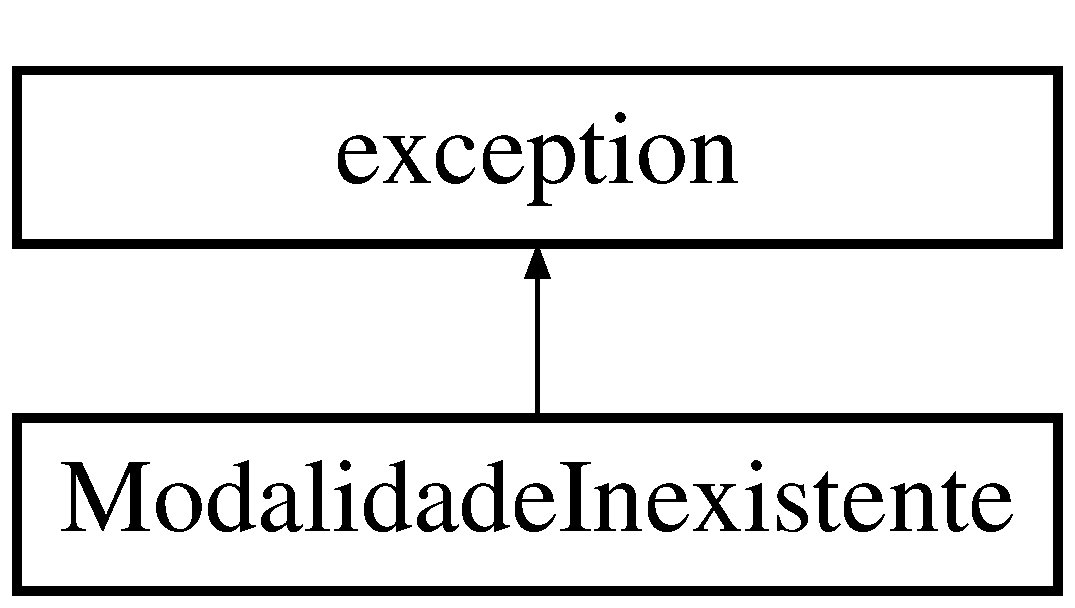
\includegraphics[height=2.000000cm]{class_modalidade_inexistente}
\end{center}
\end{figure}
\subsection*{Public Member Functions}
\begin{DoxyCompactItemize}
\item 
\hypertarget{class_modalidade_inexistente_a3eeb1f2c1dae3993ae73a016bf5119d5}{}{\bfseries Modalidade\+Inexistente} (string name\+Modality)\label{class_modalidade_inexistente_a3eeb1f2c1dae3993ae73a016bf5119d5}

\item 
\hypertarget{class_modalidade_inexistente_ac1bdf97f896db92ee136e17d38b50a9d}{}virtual const char $\ast$ {\bfseries what} () const   throw ()\label{class_modalidade_inexistente_ac1bdf97f896db92ee136e17d38b50a9d}

\end{DoxyCompactItemize}


The documentation for this class was generated from the following file\+:\begin{DoxyCompactItemize}
\item 
src/Exceptions.\+h\end{DoxyCompactItemize}

\hypertarget{class_modalidade_invalida}{}\section{Modalidade\+Invalida Class Reference}
\label{class_modalidade_invalida}\index{Modalidade\+Invalida@{Modalidade\+Invalida}}
Inheritance diagram for Modalidade\+Invalida\+:\begin{figure}[H]
\begin{center}
\leavevmode
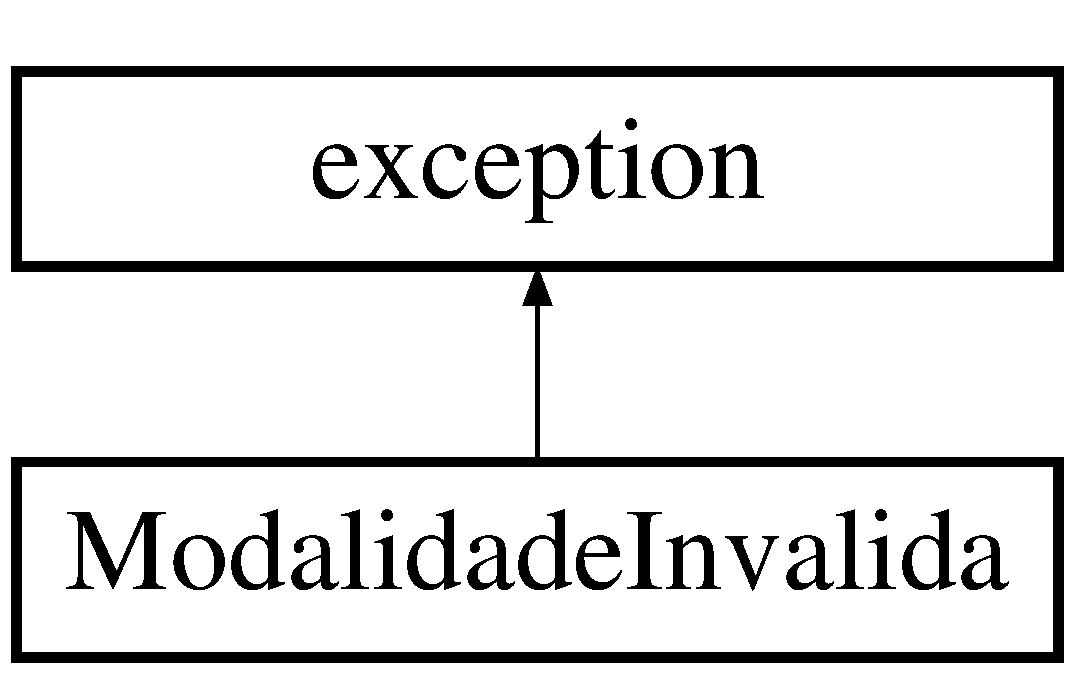
\includegraphics[height=2.000000cm]{class_modalidade_invalida}
\end{center}
\end{figure}
\subsection*{Public Member Functions}
\begin{DoxyCompactItemize}
\item 
\hypertarget{class_modalidade_invalida_a492e5df10a001077615a60d6a951bb70}{}{\bfseries Modalidade\+Invalida} (string name\+Modality, string name\+Athlete)\label{class_modalidade_invalida_a492e5df10a001077615a60d6a951bb70}

\item 
\hypertarget{class_modalidade_invalida_aa7fb2f775a9098fc9250c943e739707c}{}virtual const char $\ast$ {\bfseries what} () const   throw ()\label{class_modalidade_invalida_aa7fb2f775a9098fc9250c943e739707c}

\end{DoxyCompactItemize}


The documentation for this class was generated from the following file\+:\begin{DoxyCompactItemize}
\item 
src/Exceptions.\+h\end{DoxyCompactItemize}

\hypertarget{class_modalidade_ja_existente}{}\section{Modalidade\+Ja\+Existente Class Reference}
\label{class_modalidade_ja_existente}\index{Modalidade\+Ja\+Existente@{Modalidade\+Ja\+Existente}}
Inheritance diagram for Modalidade\+Ja\+Existente\+:\begin{figure}[H]
\begin{center}
\leavevmode
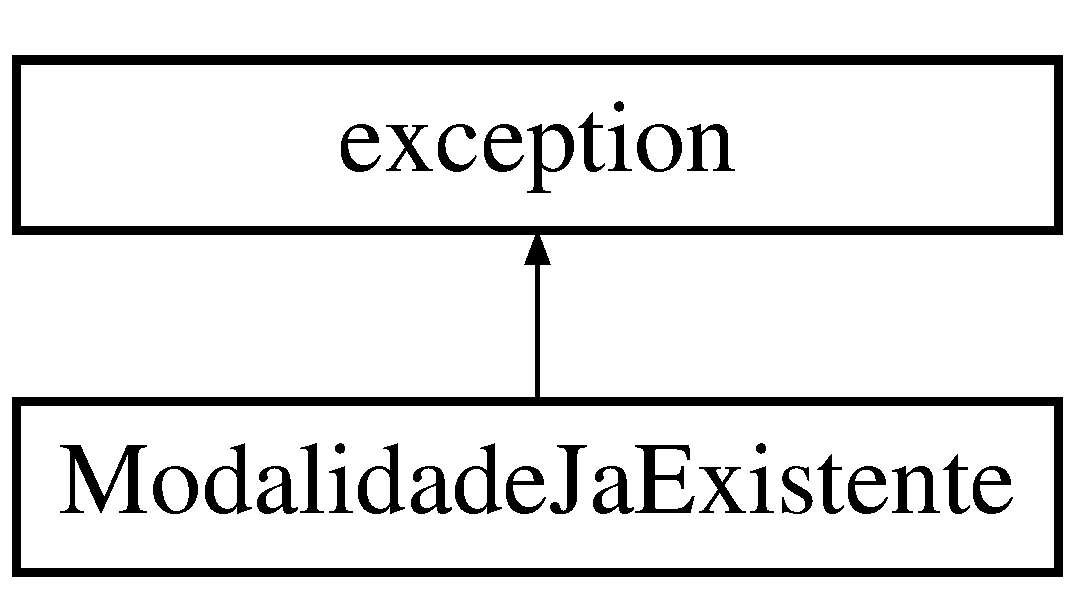
\includegraphics[height=2.000000cm]{class_modalidade_ja_existente}
\end{center}
\end{figure}
\subsection*{Public Member Functions}
\begin{DoxyCompactItemize}
\item 
\hypertarget{class_modalidade_ja_existente_a543301605276ac492f9b3764499add44}{}{\bfseries Modalidade\+Ja\+Existente} (string name\+Modality)\label{class_modalidade_ja_existente_a543301605276ac492f9b3764499add44}

\item 
\hypertarget{class_modalidade_ja_existente_a645281769ee3798058a5ab34d3e8ad53}{}virtual const char $\ast$ {\bfseries what} () const   throw ()\label{class_modalidade_ja_existente_a645281769ee3798058a5ab34d3e8ad53}

\end{DoxyCompactItemize}


The documentation for this class was generated from the following file\+:\begin{DoxyCompactItemize}
\item 
src/Exceptions.\+h\end{DoxyCompactItemize}

\hypertarget{class_num_atletas_invalido}{}\section{Num\+Atletas\+Invalido Class Reference}
\label{class_num_atletas_invalido}\index{Num\+Atletas\+Invalido@{Num\+Atletas\+Invalido}}
Inheritance diagram for Num\+Atletas\+Invalido\+:\begin{figure}[H]
\begin{center}
\leavevmode
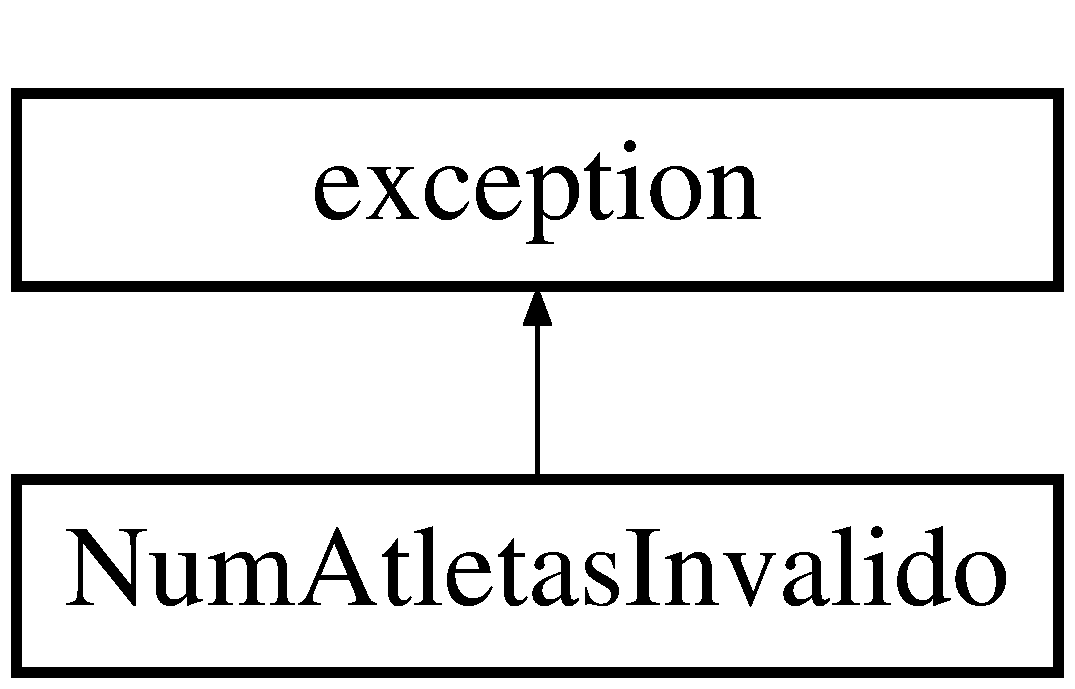
\includegraphics[height=2.000000cm]{class_num_atletas_invalido}
\end{center}
\end{figure}
\subsection*{Public Member Functions}
\begin{DoxyCompactItemize}
\item 
\hypertarget{class_num_atletas_invalido_a301bd07fd24736c82d39a2a5a1ae93ca}{}{\bfseries Num\+Atletas\+Invalido} (int num\+Athletes)\label{class_num_atletas_invalido_a301bd07fd24736c82d39a2a5a1ae93ca}

\item 
\hypertarget{class_num_atletas_invalido_a818ae652f26b2aef03e93457f7dc6a43}{}virtual const char $\ast$ {\bfseries what} () const   throw ()\label{class_num_atletas_invalido_a818ae652f26b2aef03e93457f7dc6a43}

\end{DoxyCompactItemize}


The documentation for this class was generated from the following file\+:\begin{DoxyCompactItemize}
\item 
src/Exceptions.\+h\end{DoxyCompactItemize}

\hypertarget{class_num_desportos_invalido}{}\section{Num\+Desportos\+Invalido Class Reference}
\label{class_num_desportos_invalido}\index{Num\+Desportos\+Invalido@{Num\+Desportos\+Invalido}}


{\ttfamily \#include $<$Exceptions.\+h$>$}

Inheritance diagram for Num\+Desportos\+Invalido\+:\begin{figure}[H]
\begin{center}
\leavevmode
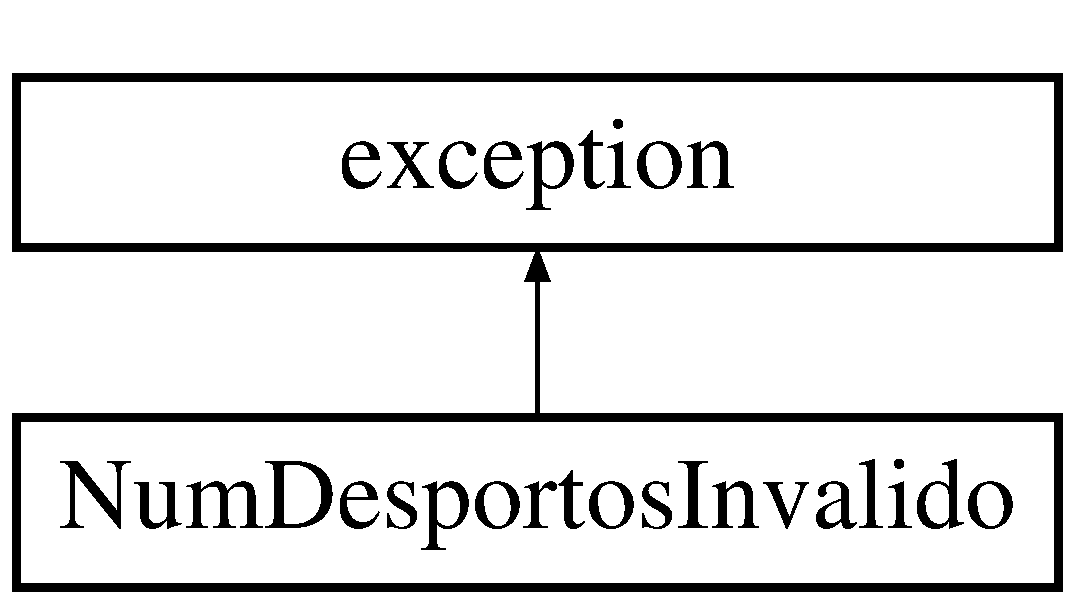
\includegraphics[height=2.000000cm]{class_num_desportos_invalido}
\end{center}
\end{figure}
\subsection*{Public Member Functions}
\begin{DoxyCompactItemize}
\item 
\hypertarget{class_num_desportos_invalido_abe15254e061c4663cd9a9131b17a974f}{}{\bfseries Num\+Desportos\+Invalido} (int num\+Sports\+Max)\label{class_num_desportos_invalido_abe15254e061c4663cd9a9131b17a974f}

\item 
\hypertarget{class_num_desportos_invalido_a66807c7bcc9a349c703649e8de61681d}{}virtual const char $\ast$ {\bfseries what} () const   throw ()\label{class_num_desportos_invalido_a66807c7bcc9a349c703649e8de61681d}

\end{DoxyCompactItemize}


\subsection{Detailed Description}
E\+X\+C\+E��\+E\+S N\+U\+M\+I\+N\+V\+A\+L\+I\+D\+O 

The documentation for this class was generated from the following file\+:\begin{DoxyCompactItemize}
\item 
src/Exceptions.\+h\end{DoxyCompactItemize}

\hypertarget{class_num_modalidades_invalido}{}\section{Num\+Modalidades\+Invalido Class Reference}
\label{class_num_modalidades_invalido}\index{Num\+Modalidades\+Invalido@{Num\+Modalidades\+Invalido}}
Inheritance diagram for Num\+Modalidades\+Invalido\+:\begin{figure}[H]
\begin{center}
\leavevmode
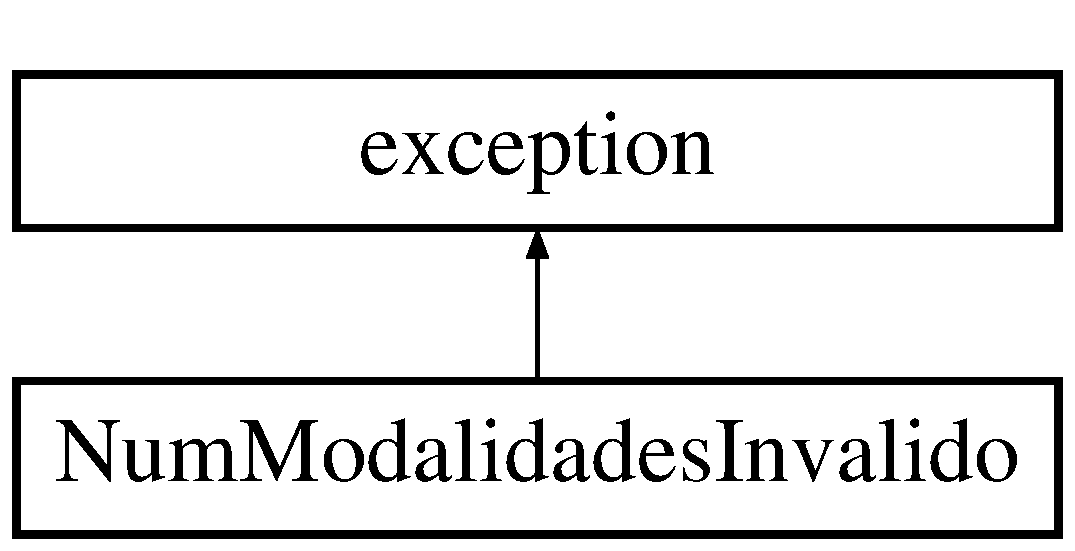
\includegraphics[height=2.000000cm]{class_num_modalidades_invalido}
\end{center}
\end{figure}
\subsection*{Public Member Functions}
\begin{DoxyCompactItemize}
\item 
\hypertarget{class_num_modalidades_invalido_afd6000e26dddd366ab91f604d312c597}{}virtual const char $\ast$ {\bfseries what} () const   throw ()\label{class_num_modalidades_invalido_afd6000e26dddd366ab91f604d312c597}

\end{DoxyCompactItemize}


The documentation for this class was generated from the following file\+:\begin{DoxyCompactItemize}
\item 
src/Exceptions.\+h\end{DoxyCompactItemize}

\hypertarget{class_pessoa}{}\section{Pessoa Class Reference}
\label{class_pessoa}\index{Pessoa@{Pessoa}}
Inheritance diagram for Pessoa\+:\begin{figure}[H]
\begin{center}
\leavevmode
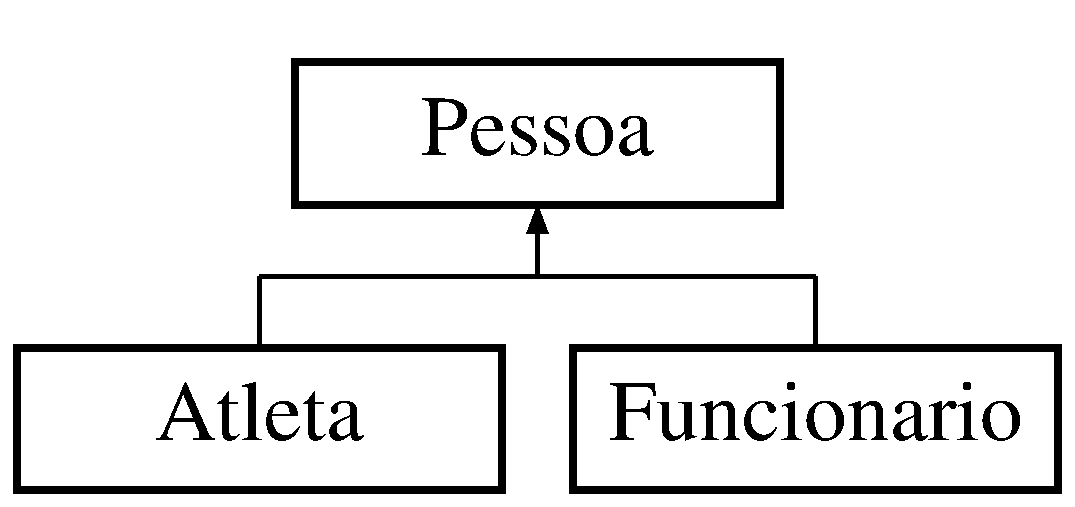
\includegraphics[height=2.000000cm]{class_pessoa}
\end{center}
\end{figure}
\subsection*{Public Member Functions}
\begin{DoxyCompactItemize}
\item 
\hypertarget{class_pessoa_a0d11e4a70a79133099518b53f93b05cd}{}{\bfseries Pessoa} (string name, unsigned int age)\label{class_pessoa_a0d11e4a70a79133099518b53f93b05cd}

\item 
\hypertarget{class_pessoa_a8d4d2f40ba5634f49b0ce181fee7f0a7}{}string {\bfseries get\+Nome} () const \label{class_pessoa_a8d4d2f40ba5634f49b0ce181fee7f0a7}

\item 
\hypertarget{class_pessoa_a68115ff0ae1e9d73a87beb4a89c2cd93}{}unsigned int {\bfseries get\+Idade} () const \label{class_pessoa_a68115ff0ae1e9d73a87beb4a89c2cd93}

\item 
\hypertarget{class_pessoa_a3a0b84de86eb7640915a332be964812f}{}virtual void {\bfseries info} ()=0\label{class_pessoa_a3a0b84de86eb7640915a332be964812f}

\end{DoxyCompactItemize}


The documentation for this class was generated from the following files\+:\begin{DoxyCompactItemize}
\item 
src/Pessoa.\+h\item 
src/Pessoa.\+cpp\end{DoxyCompactItemize}

\hypertarget{class_prova}{}\section{Prova Class Reference}
\label{class_prova}\index{Prova@{Prova}}
\subsection*{Public Member Functions}
\begin{DoxyCompactItemize}
\item 
\hypertarget{class_prova_acb142e2a5d1208413d18b2a82a0b091b}{}{\bfseries Prova} (string name, int day, int month, int year)\label{class_prova_acb142e2a5d1208413d18b2a82a0b091b}

\item 
\hypertarget{class_prova_a36e205bd3a124c2ec00f0391ecb7fdfd}{}string {\bfseries get\+Nome} () const \label{class_prova_a36e205bd3a124c2ec00f0391ecb7fdfd}

\item 
\hypertarget{class_prova_a320a56d0682344bfc42d3522222e04d6}{}int {\bfseries get\+Ano} () const \label{class_prova_a320a56d0682344bfc42d3522222e04d6}

\item 
\hypertarget{class_prova_af73d2143f0a524458e4bea47144051ea}{}int {\bfseries get\+Mes} () const \label{class_prova_af73d2143f0a524458e4bea47144051ea}

\item 
\hypertarget{class_prova_a4937a86197edcd21ab27f24bb19bf5e6}{}int {\bfseries get\+Dia} () const \label{class_prova_a4937a86197edcd21ab27f24bb19bf5e6}

\item 
\hypertarget{class_prova_aaa98c4af9413dcbef62b746211392319}{}\hyperlink{class_modalidade}{Modalidade} $\ast$ {\bfseries get\+Modalidade} ()\label{class_prova_aaa98c4af9413dcbef62b746211392319}

\item 
\hypertarget{class_prova_a7c2ceb8e87016ffc1664ff2d6bf9fdfc}{}map$<$ \hyperlink{class_atleta}{Atleta} $\ast$, int $>$ {\bfseries get\+Classificacoes\+Atletas} ()\label{class_prova_a7c2ceb8e87016ffc1664ff2d6bf9fdfc}

\item 
\hypertarget{class_prova_ade85a788f4ad45311315e1f7d59b74bd}{}\hyperlink{class_infrastrutura}{Infrastrutura} $\ast$ {\bfseries get\+Infrastrutura} ()\label{class_prova_ade85a788f4ad45311315e1f7d59b74bd}

\item 
\hypertarget{class_prova_af264957eb89840e0c50ba9d1715efa08}{}void {\bfseries set\+Modalidade} (\hyperlink{class_modalidade}{Modalidade} $\ast$mod)\label{class_prova_af264957eb89840e0c50ba9d1715efa08}

\item 
\hypertarget{class_prova_a24499b4bd41c7e72098325e984d20a86}{}void {\bfseries set\+Infrastrutura} (\hyperlink{class_infrastrutura}{Infrastrutura} $\ast$infra)\label{class_prova_a24499b4bd41c7e72098325e984d20a86}

\item 
\hypertarget{class_prova_ae2b612d5e23720e7ce7d48d7fba7db63}{}void {\bfseries set\+Classificacoes\+Atletas} (map$<$ \hyperlink{class_atleta}{Atleta} $\ast$, int $>$ map)\label{class_prova_ae2b612d5e23720e7ce7d48d7fba7db63}

\end{DoxyCompactItemize}


The documentation for this class was generated from the following files\+:\begin{DoxyCompactItemize}
\item 
src/Prova.\+h\item 
src/Prova.\+cpp\end{DoxyCompactItemize}

\hypertarget{class_prova_inexistente}{}\section{Prova\+Inexistente Class Reference}
\label{class_prova_inexistente}\index{Prova\+Inexistente@{Prova\+Inexistente}}
Inheritance diagram for Prova\+Inexistente\+:\begin{figure}[H]
\begin{center}
\leavevmode
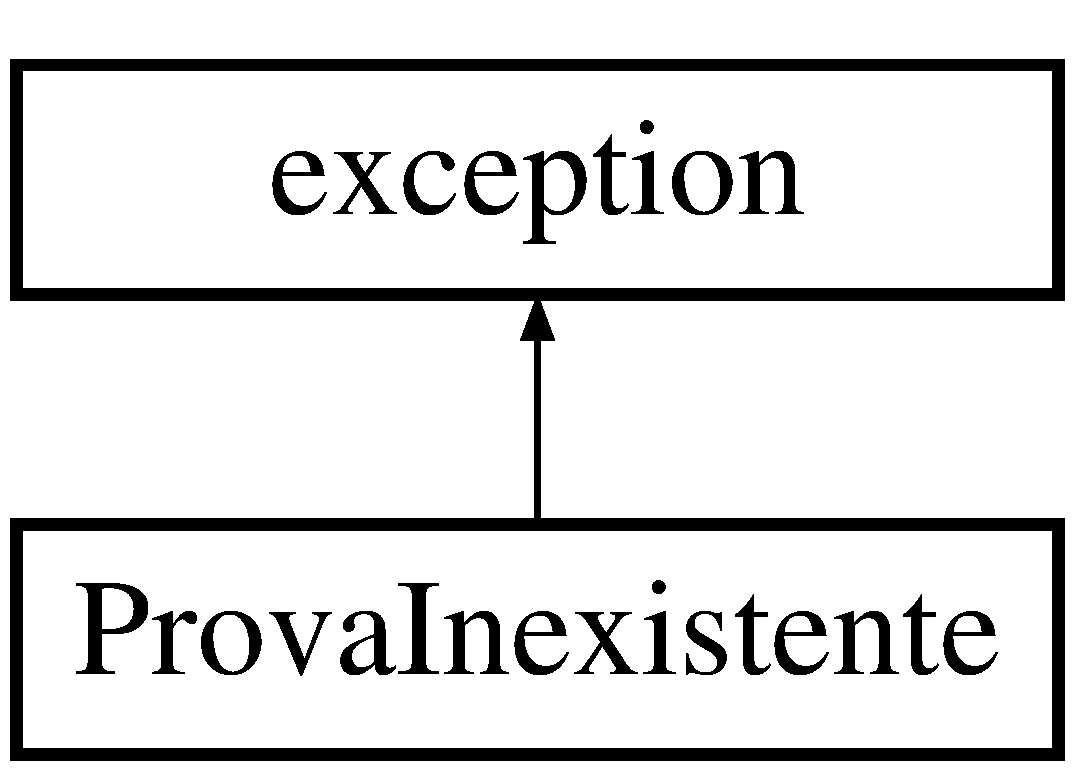
\includegraphics[height=2.000000cm]{class_prova_inexistente}
\end{center}
\end{figure}
\subsection*{Public Member Functions}
\begin{DoxyCompactItemize}
\item 
\hypertarget{class_prova_inexistente_a28509bb7a080cf2d487ab1061ff5f539}{}{\bfseries Prova\+Inexistente} (string name\+Match)\label{class_prova_inexistente_a28509bb7a080cf2d487ab1061ff5f539}

\item 
\hypertarget{class_prova_inexistente_ae8a129d3e086d1e43f4797918037db46}{}virtual const char $\ast$ {\bfseries what} () const   throw ()\label{class_prova_inexistente_ae8a129d3e086d1e43f4797918037db46}

\end{DoxyCompactItemize}


The documentation for this class was generated from the following file\+:\begin{DoxyCompactItemize}
\item 
src/Exceptions.\+h\end{DoxyCompactItemize}

\hypertarget{class_prova_ja_existente}{}\section{Prova\+Ja\+Existente Class Reference}
\label{class_prova_ja_existente}\index{Prova\+Ja\+Existente@{Prova\+Ja\+Existente}}
Inheritance diagram for Prova\+Ja\+Existente\+:\begin{figure}[H]
\begin{center}
\leavevmode
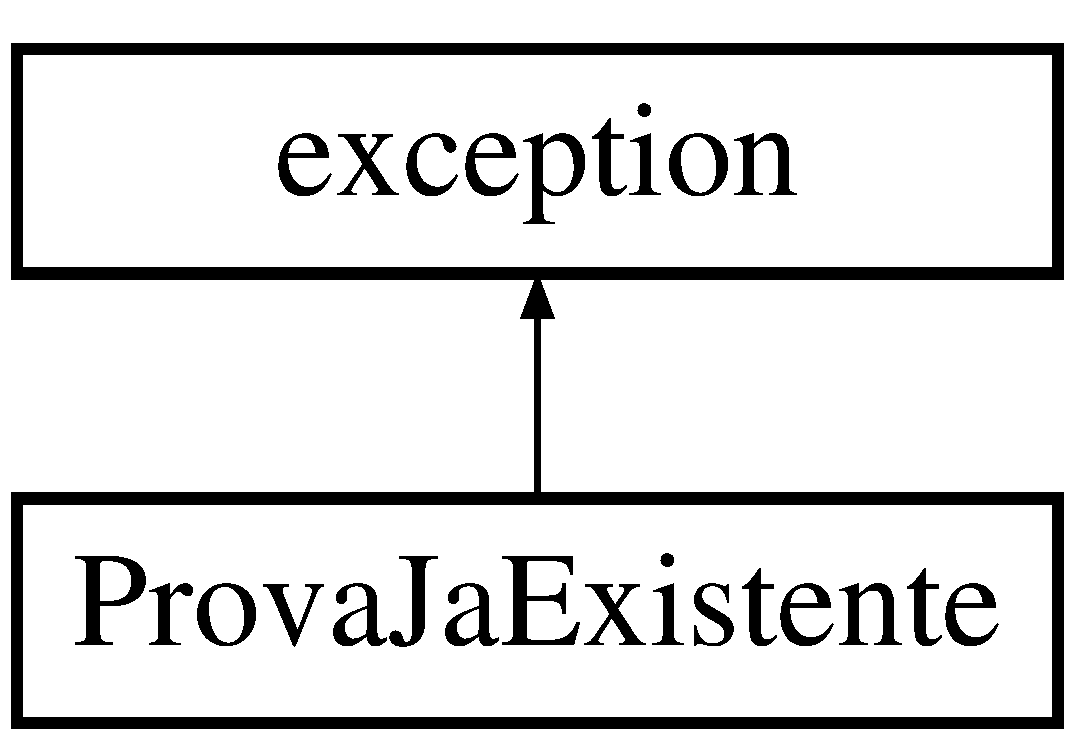
\includegraphics[height=2.000000cm]{class_prova_ja_existente}
\end{center}
\end{figure}
\subsection*{Public Member Functions}
\begin{DoxyCompactItemize}
\item 
\hypertarget{class_prova_ja_existente_a06725a8d51855c01a51647b54320db51}{}{\bfseries Prova\+Ja\+Existente} (string name\+Match)\label{class_prova_ja_existente_a06725a8d51855c01a51647b54320db51}

\item 
\hypertarget{class_prova_ja_existente_a04840dd71409c57e714da57fee392beb}{}virtual const char $\ast$ {\bfseries what} () const   throw ()\label{class_prova_ja_existente_a04840dd71409c57e714da57fee392beb}

\end{DoxyCompactItemize}


The documentation for this class was generated from the following file\+:\begin{DoxyCompactItemize}
\item 
src/Exceptions.\+h\end{DoxyCompactItemize}

%--- End generated contents ---

% Index
\backmatter
\newpage
\phantomsection
\clearemptydoublepage
\addcontentsline{toc}{chapter}{Index}
\printindex

\end{document}
